% Modified from AAAS Science LATEX template
% Use only LaTeX2e, calling the article.cls class and 12-point type.

\documentclass[10pt, oneside]{article}

\usepackage{helvet}
\renewcommand{\familydefault}{\sfdefault}
\usepackage{graphicx}
\usepackage{caption}
\usepackage{float}
\captionsetup{font=small}
\usepackage{textcomp}
\usepackage{url}
\usepackage{cite}
\usepackage{nameref}
\usepackage[none]{hyphenat}%%%%
\usepackage[utf8]{inputenc}
\usepackage[english]{babel}
\usepackage[T1]{fontenc}
\usepackage{multicol}
\setlength{\columnsep}{0.5cm}
\usepackage{titlesec}

\titleformat*{\section}{\large\bfseries}
\titleformat*{\subsection}{\normalsize\bfseries}
\titleformat*{\subsubsection}{\normalsize\bfseries}

% Page setup
\topmargin -2cm
\oddsidemargin -1cm
\evensidemargin 1cm
\textwidth 18cm
\textheight 24cm
\footskip 1.0cm


\newcommand{\beginsupplement}{%
  \setcounter{table}{0}
  \renewcommand{\thetable}{S\arabic{table}}%
  \setcounter{figure}{0}
  \renewcommand{\thefigure}{S\arabic{figure}}%
}

% Include the date command, but leave its argument blank to prevent date print.
\date{}

%%%%%%%%%%%%%%%%% END OF PREAMBLE %%%%%%%%%%%%%%%%

% Initialize use of code blocks with syntax highlighting
\usepackage{listings}
\usepackage{color}

\definecolor{dkgreen}{rgb}{0,0.6,0}
\definecolor{gray}{rgb}{0.5,0.5,0.5}
\definecolor{mauve}{rgb}{0.58,0,0.82}

\lstset{frame=tb,
  language=Java,
  aboveskip=3mm,
  belowskip=3mm,
  showstringspaces=false,
  columns=flexible,
  basicstyle={\small\ttfamily},
  numbers=none,
  numberstyle=\tiny\color{gray},
  keywordstyle=\color{blue},
  commentstyle=\color{dkgreen},
  stringstyle=\color{mauve},
  breaklines=true,
  breakatwhitespace=true,
  tabsize=3
}

%%%%%%%%%%%%%%%%% START OF DOCUMENT %%%%%%%%%%%%%%%%

\begin{document}

% Paper title
\noindent
{\huge
\textbf{XPRESSyourself: Enhancing, Standardizing, and \\
Automating Ribosome Profiling Computational \\
Analyses Yields Improved Insight into Data
}
}

\bigskip

% Author info

% Author list/order:
\noindent
{\large
\textbf{Jordan A. Berg,$^{1\ast}$ Jonathan R. Belyeu,$^{2}$ Jeffrey T. Morgan,$^{1}$ Alex J. Bott,$^{1}$ Yeyun Ouyang,$^{1}$ Aaron R. Quinlan,$^{2,4,5}$ Jason Gertz,$^{3}$ Jared Rutter$^{1,6\ast}$
}
} \\

\noindent
{$^{1}$Department of Biochemistry, University of Utah, Salt Lake City, UT, USA, 84112.}
{$^{2}$Department of Human Genetics, University of Utah, Salt Lake City, UT, USA, 84112.}
{$^{3}$Department of Oncological Sciences, University of Utah, Salt Lake City, UT, USA, 84112.}
{$^{4}$USTAR Center for Genetic Discovery, University of Utah, Salt Lake City, UT, USA, 84112.}
{$^{5}$Department of Biomedical Informatics, University of Utah, Salt Lake City, UT, USA, 84112.}
{$^{6}$Howard Hughes Medical Institute, University of Utah, Salt Lake City, UT, USA, 84112.}\\
{$^\ast$Address correspondence to: jordan.berg@biochem.utah.edu, rutter@biochem.utah.edu}

\bigskip

% Abstract
\noindent
\textbf{Ribosome profiling, an application of nucleic acid sequencing for monitoring ribosome activity, has \\revolutionized our understanding of protein translation dynamics. This technique has been available for a decade, yet the current state of publicly available computational tools for these data is bleak. We introduce XPRESSyourself, an analytical toolkit that eliminates barriers and bottlenecks associated with this specialized data type by filling gaps in the computational toolset for both experts and non-experts of ribosome profiling. It also automates and standardizes analysis procedures, decreasing time-to-discovery and increasing \\reproducibility. We demonstrate this toolkit's performance on publicly available ribosome profiling data and associated bulk RNA-Seq data by rapidly identifying hypothetical mechanisms related to neurodegenerative phenotypes and neuroprotective mechanisms of the small-molecule ISRIB during acute cellular stress. \\XPRESSyourself brings robust, rapid analysis of ribosome-profiling data to a broad and ever-expanding audience and will lead to more reproducible and accessible measurements of translation regulation. The XPRESSyourself software is perpetually open-source and is hosted at https://github.com/XPRESSyourself.
}

\setlength{\parindent}{2em}

%\section*{Keywords}
%Ribosome Profiling, RNA-Seq, Standardized, Automated, Analysis, GTF Truncation, rRNA depletion, Intron-agnostic Gene Coverage, Transcriptome-wide Metagene Assessment

\begin{multicols}{2}


\section*{Introduction}
High-throughput sequencing data has revolutionized biomedical and biological research. One such application of this consequential technology is ribosome profiling, which, coupled with bulk RNA-Seq, measures translation efficiency, translation pausing, novel protein translation products, and more. \cite{ingolia_science, riboseq_overview, ingolia_meth}. Though ribosome profiling has matured, there remains an abundance of biases and peculiarities associated with each analytical method or tool, which are often obscured to a user. Very few labs have the tools to separate the biological signals in ribosome-profiling data from inherent biases of the experimental measurements, and these tools are not readily accessible by the community. This is a critical time in the rapidly expanding life of ribosome-footprint profiling. For too long, the bioinformatic know-how of this incredibly powerful technique has been limited to a small handful of labs. As more and more ribosome profiling studies are performed, more and more labs will lack the ability to analyze their data with ease and fidelity. Few if any extant pipelines or toolkits offer a thorough set of integrated tools for assessing standard quality control metrics or performing proper reference curation across any organism, particularly with ribosome profiling data \cite{galaxy, ribogalaxy, nextflow_pipeline, dnanexus_pipeline, riboviz}. \par

For example, the pile-up of ribosomes at the $5'$- and $3'$- ends of coding regions within a transcript is a systematic biological artifact arising from the slower kinetics of ribosome initiation and termination compared to translation elongation and is often not relevant to measurements of translation regulation \cite{gerashchenko_nar, artieri_gr, hussman_plosg}. These pile-ups can dramatically skew ribosome footprint quantification and measurements of translational efficiency. Experts generally recommend excluding these pile-up-prone regions when quantifying ribosome profiling alignments \cite{ingolia_meth, weinberg_reports}; however, no publicly available computational tools currently exist to facilitate these automated adjustments to reference transcripts. In addition, downstream data visualization methods presently available are not optimized or even able to quantify and compare only those transcriptional regions relevant to translational regulation. \par

We developed XPRESSyourself, a computational toolkit and pipeline that bridges these and other gaps in ribosome profiling analysis. XPRESSyourself implements the complete suite of tools necessary for ribosome-profiling and bulk RNA-Seq analysis in a robust and easy-to-use software package. This software will lead to more reproducible and more accessible measurements of translation regulation. For instance, XPRESSyourself creates the mRNA-annotation files necessary to remove confounding systematic factors from quantification and analysis of ribosome profiling data to measure translation accurately. It also provides a built-in capacity to quantify and visualize differential upstream open-reading frame (uORF) usage. The ability to visualize (and in another XPRESSyourself module, quantify) the usage of micro-uORFs is important in exploring regulatory events or mechanisms in a wide array of biological responses and diseases. \par

An additional tool introduced in XPRESSyourself surveys sequence libraries for problematic rRNAs. rRNA depletion is intrinsically complicated during the preparation of ribosome-footprint profiling libraries: poly(A) selection is irrelevant, and kit-based rRNA depletion is grossly insufficient. Depending on the species and condition being profiled, a small subset of rRNA fragments (generally 2-5) can easily account for more than 90\% of sequenced reads. XPRESSyourself introduces a tool for efficient identification of the most problematic rRNA fragments for targeted depletion, which provides immense financial and experimental benefits to the user as ribosome footprint signal can be better amplified over rRNA noise. \par

XPRESSyourself aims to address the lack of consensus in analytical approaches used to process ribosome profiling and other RNA-Seq data. For example, while a basic bioinformatic understanding is more commonplace amongst scientists, the intricacies of processing RNA-Seq data remain challenging for many. Moreover, many users are often not aware of the most up-to-date tools or the appropriate settings for their application \cite{costello_npjsba, funari_science}. Even for the experienced user, developing robust automated pipelines that accurately process and assess the quality of these datasets can be laborious. The variability that inevitably arises with each lab or core facility designing and using distinct pipelines is also a challenge to the field. \par

XPRESSyourself provides an accessible, simple-to-use, automated analysis platform for RNA-Seq, often packaging tasks that would typically require hundreds to thousands of lines of code into a single command. XPRESSyourself curates the state-of-the-art methods for use and where a required functionality is unavailable, introduces a thoroughly tested module to fill that gap. In addition to the new tools described above, the toolkit provides the user with a complete suite of software to handle pre-processing, aligning, and quantifying of sequence reads, performing quality control via various meta-analyses of pre- and post-processed reads. We also provide access to key quality control measurements useful for assessing ribosome profiling and other RNA-Seq experiments. These include read length distribution plots that are particularly helpful for ribosome profiling experiments due to the unique characteristics of the ribosome footprint-sized libraries (usually around 17-33 nucleotides) \cite{fp_range}, and a periodicity sub-module that tracks the P-site of ribosome footprints to assess effective capture of the characteristic one codon step of the ribosome. XPRESSpipe also includes a metagene analysis sub-module that shows the distribution of the relative position of all aligned reads across a representative transcript to help identify any $5'$- or $3'$- biases in RNA fragment capture during library preparation. Additionally, XPRESSpipe includes a module for plotting gene coverage, similar to interactive genome browser programs, such as IGV \cite{igv}, but where introns are collapsed to more clearly visualize read coverage across exons or coding space. As PCR-based duplicate biases can arise during sequence library preparation, a library complexity visualization sub-module is included in the pipeline to assess the frequency of PCR amplification artifacts in the library and ensure appropriately broad coverage of gene population was captured during sequence library creation. \par

Finally, the most broadly relevant aspect of our update and streamlining of ribosome-profiling analysis is the novel biological insights we are able to obtain from published datasets. We highlight this in the ISRIB ribosome-profiling study, where we are able to observe significant translation regulation that was missed previously when the data were initially analyzed using now outdated techniques. This analysis generates novel hypotheses for genes potentially involved in neurodegeneration in humans, but more broadly emphasizes the benefit of analysis and re-analysis of data using the up-to-date and benchmarked methodology provided within XPRESSyourself.

\section*{Results}

\subsection*{Architecture and Organization}
XPRESSyourself is currently partitioned into two software packages, XPRESSpipe and XPRESSplot. XPRESSpipe contains automated pipelines tailored for ribosome profiling, single-end RNA-Seq, and paired-end RNA-Seq datasets. Required reference files are FASTA files and the appropriate GTF file saved as \texttt{transcripts.gtf}. We recommend that these reference files are obtained from Ensembl \cite{ensembl}. Input data are generally FASTQ-formatted files, and outputs will vary from FASTQ to BAM files, or PDF files for quality control outputs. \par

The pipelines handle pre-processing, alignment, and quantification of sequencing reads, after which it will perform essential quality control analyses of each sequence library. We will focus on ribosome profiling examples to demonstrate the utility of XPRESSpipe, while the majority of statements are also applicable to general single- or paired-end RNA-Seq. Individual sub-modules can be run automatically through a pipeline or manually. Processes modulate settings to optimize available computational resources to deliver results as quickly as possible. XPRESSplot is available as a Python library and provides an array of plotting methods specifically for sequence data, but tractable to other data types. More details can be found in each package's documentation \cite{xpresspipe_docs, xpressplot_docs}. \par

For nearly all sub-modules, log files are written to the provided output directory to summarize provided user parameters, track performance, and report errors. An additional log file is written summarizing the versions of the different dependency software used during the execution of the pipeline or sub-module. Users are encouraged to provide these files as supplements within publications when presenting XPRESSpipe-processed data to aid in documentation.

The software is designed such that updating and testing of a new module, or updating dependency usage, are facile tasks for a trained bioinformatician.

\subsection*{Installation and Usability}
XPRESSyourself suite packages can be easily installed following directions and/or walkthrough videos provided in the documentation and READMEs \cite{xpressyourself, xpresspipe_docs, xpressplot_docs}. \par

XPRESSyourself aims to make ribosome profiling and sequence analysis as easy and accessible as possible to all users. As such, an integrated command builder for reference curation and sample analysis can be run by executing \texttt{xpresspipe build}. This command builder will walk the user through potential considerations based on their library preparation method and build the appropriate command for execution on their personal computer or a supercomputing cluster. If running the command builder on a personal machine, the user can then have XPRESSpipe execute the command automatically. In addition to this resource, the XPRESSyourself suite provides thorough documentation for each module and tool, along with video walkthroughs (accessible through the README files) and interactive notebooks (found in the home directory of a package.

\subsection*{Automated Reference Curation}
The first step of RNA-Seq alignment is curating an organism reference to which the alignment software will map reads. XPRESSpipe uses STAR \cite{star} for mapping reads as it has been shown consistently to be the best performing read aligner for RNA-Seq data \cite{alignment_benchmark}. The appropriate reference files are automatically curated by providing the appropriate GTF file saved as \texttt{transcripts.gtf} and the directory path to the genomic FASTA file(s). Additional modifications to the GTF file required for ribosome profiling are discussed in the next section.


\subsection*{GTF Modification}
For ribosome profiling, we observe frequent read pile-ups at the $5'$- and $3'$- ends of an open reading frame which are largely uninformative as to the translational efficiency of the gene. Therefore, the $5'$- and $3'$- ends of each transcript's total coding region should be truncated as to be excluded from consideration during read quantification \cite{ingolia_meth, weinberg_reports}. By providing the \texttt{-{}-truncate} argument, as shown above, the $5'$- and $3'$- ends of each coding region will be trimmed by the specified amounts. These values are set to defaults of 45 nt for $5'$- truncation and 15 nt for $3'$- truncation, as is the convention within the ribosome profiling field \cite{ingolia_meth}, but these can be modified using the \texttt{-{}-truncate\_5prime} or \texttt{-{}-truncate\_3prime} parameters. If generating a GTF for use with general RNA-Seq datasets not associated with a ribosome profiling dataset (i.e., an RNA-Seq library that originates from the same sample as a ribosome profiling library), the \texttt{-{}-truncate} argument should not be provided. \par

Additional parameters that can be used during this step include \texttt{-{}-protein\_coding} and \texttt{-{}-longest\_transcript}. By providing the \texttt{-{}-protein\_coding} argument, as shown above, only protein-coding genes are retained in the GTF file. As ribosomal RNAs and other non-coding RNAs can be highly abundant in RNA-Seq experiments, it is often recommended to not include these sequences for quantification. This acts as a read masking step to exclude non-protein coding transcripts from downstream analyses. By providing the \texttt{-{}-longest\_transcript} argument, the longest Ensembl canonical transcript \cite{ensembl_canon} is retained for each gene in the GTF file. In most eukaryotes, mRNAs undergo alternative splicing of exons to generate the mature mRNA. However, some tools consider reads that align to multiple annotated splice variants of a gene as a multi-mapping read since they map to a location where several isoforms, recognized as separate records, of the same gene overlap. These reads are either penalized or discarded. However, if using HTSeq with default XPRESSpipe parameters or Cufflinks to quantify reads, this is not necessary as the software is optimized to quantify abundances of the different isoforms of each gene \cite{cufflinks}. \par

\subsection*{Read Processing}
\textbf{Pre-Processing}. In order for sequence reads to be mapped to the genome, reads generally need to be cleaned of artifacts from library creation. These include adaptors, unique molecular identifier (UMI) sequences, and technical errors in the form of low-quality base calls. Parameters, like minimum acceptable quality or length, can be modified, or features like UMIs can be added to identified and grouped for later removal of PCR artifacts \cite{umi, umitools}. \par

\noindent\textbf{Mapping}. Reads are aligned to the reference genome, using STAR, which, despite being more memory-intensive, is relatively fast and one of the most accurate sequence alignment options currently available \cite{star, baruzzo_natmeth}. XPRESSpipe is capable of performing a single-pass, splice-aware, GTF-guided alignment or a two-pass alignment of reads wherein novel splice junctions are determined and built into the reference, followed by alignment of reads to the new reference. A coordinate-sorted and indexed BAM file is output by STAR. We abstain from rRNA negative alignment at this step as downstream analysis of these mapped reads could be of interest to some users. \par

\noindent\textbf{Quantification}. XPRESSpipe further processes alignment files by optionally parsing for unique alignments that are then passed on to the next steps. PCR duplicates are detected and marked or removed for downstream processing; however, these files are only used for relevant downstream steps (such as library complexity quality control) or if the user specifies to use these de-duplicated files in downstream steps such as read quantification. Use of de-duplicated alignment files may be advisable in situations where the library complexity profiles (discussed below) exhibit high duplication frequencies. However, generally the abundance of PCR-duplicates is low in properly-prepared sequencing libraries; thus, doing so may be overly stringent and unnecessary \cite{umi}. Optionally, BED coverage files can also be output. \par

\noindent\textbf{Post-Processing}. XPRESSpipe quantifies read alignments for each input file using HTSeq with the \texttt{intersection-nonempty} method by default \cite{htseq, count_benchmark}. Our rationale for including this quantification method is that it conforms to the current default TCGA standards and is favorable in most applications. If masking of non-coding RNAs is desired, a \texttt{protein\_coding} modified GTF file should be provided for the \texttt{-{}-gtf} argument. HTSeq is recommended for processing ribosome profiling data as it allows selection of feature type across which to quantify, thus allowing for quantification across the CDSs of a transcript instead of the exons. Additionally, if a user is interested in quantifying ribosome occupancy of transcript uORFs for ribosome footprint samples, they could provide \texttt{five\_prime\_utr} or \texttt{three\_prime\_utr} for the \texttt{-{}-feature\_type} parameter if such annotations exist for the organism of interest. If the user is interested in isoform abundance estimation, Cufflinks is available to perform this method of quantification instead \cite{cufflinks, count_benchmark}. \par

\noindent\textbf{Normalization}. Methods for count normalization are available within XPRESSpipe by way of the XPRESSplot package. For normalizations correcting for transcript length, the appropriate GTF must be provided. Current sample normalization methods available include reads-per-million (RPM), Reads-per-kilobase-million (RPKM) or Fragments-per-kilobase-million (FPKM), and transcripts per million (TPM) normalization \cite{evans_briefbio}. For samples sequenced on different flow cells, prepared by different individuals, or on different days, the \texttt{-{}-batch} argument should be provided along with the appropriate metadata matrix, which is then processed by way of XPRESSplot using the ComBat package \cite{sva}. \par

\subsection*{Quality Control}
\textbf{Read Length Distribution}. The lengths of all reads are analyzed after trimming. By assessing the read distribution of each sample, the user can ensure the expected read size was sequenced. This is particularly helpful in ribosome profiling experiments for verifying the requisite 17-33 nt ribosome footprints were selectively captured during library preparation \cite{ingolia_meth, fp_range}. Metrics here, as in all other quality control sub-modules, are then compiled into summary figures by XPRESSpipe for assessment of the overall experiment by the user. \par

\noindent\textbf{Library Complexity}. Measuring library complexity is an effective method for analyzing the robustness of a sequencing experiment in capturing various, unique RNA species. As the majority of RNA-Seq preparation methods involve a PCR step, sometimes particular fragments will be favored and over-amplified in contrast to others. By plotting the number of PCR replicates versus expression level for each gene, one can monitor any effects of limited transcript capture diversity and/or high estimated PCR duplication rate on the robustness of their libraries. This analysis is performed using dupRadar \cite{dupradar} where inputs are PCR duplicate-tagged BAM files output. Metrics are then compiled and plotted by XPRESSpipe. \par

\noindent\textbf{Metagene Estimation Profile}. To identify any general biases for the preferential capture of the $5'$- or $3'$- ends of transcripts, metagene profiles can be generated for each sample. This is performed by determining the meta-genomic coordinate for each aligned read in exon space. Required inputs are an indexed BAM file and an un-modified GTF reference file. Outputs include metagene metrics, individual plots, and summary plots. If desired, a meta-profile across a representative CDS can be performed. \par

\noindent\textbf{Gene Coverage Profile}. Extending the metagene estimation analysis, the user can focus on the coverage profile across a single gene. Although traditional tools like IGV \cite{igv} offer the ability to perform such tasks, XPRESSpipe provides the ability to collapse the introns to observe coverage over exon space only. This is helpful in situations where massive introns spread out exons and make it difficult to visualize exon coverage for the entire transcript in a concise manner. When running an XPRESSpipe pipeline, a housekeeping gene will be processed and output for the user's reference. Figure \ref{fig:supplement1} provides a comparison with the output of IGV \cite{igv} and XPRESSpipe's geneCoverage module over a similar region for two genes to demonstrate the compatibility between the methods. \par

\noindent\textbf{Codon Phasing/Periodicity Estimation Profile}. In ribosome profiling, a useful measure of a successful experiment comes by investigating the codon phasing of ribosome footprints \cite{ingolia_meth}. To do so, the P-site positions relative to the start codon of each ribosome footprint that mapped to a transcript are calculated using riboWaltz \cite{ribowaltz}. The same inputs are required as in the \texttt{metagene} sub-module. \par

\noindent\textbf{Identify Problematic rRNA Fragments from Ribosome Footprinting for Depletion}. Ribosomal RNA (rRNA) contamination is common in RNA-Seq library preparation as the bulk of RNA in a cell is dedicated to rRNA. The sequencing of these RNAs becomes highly repetitive, wasteful, and typically biologically uninteresting in the context of gene expression and translation efficiency. The depletion of these sequences is therefore desired to increase the depth of coverage of ribosome footprints. To facilitate this depletion, many commercial kits are available that target specific rRNA sequences for depletion or that enrich for poly(A)-tailed mRNAs. However, and especially in the case of ribosome profiling experiments, where RNA is digested by an RNase to create ribosome footprints, many commercial depletion kits will not target the most abundant rRNA fragment species produces during the footprinting step of ribosome profiling. Poly(A)-selection kits are inappropriate as footprints will not have the requisite poly(A) tail. To this end, custom rRNA-depletion probes are recommended \cite{ingolia_meth, ingolia_science}. \texttt{rrnaProbe} analyzes the over-represented sequences within a collection of footprint libraries that have already undergone adaptor and quality trimming, compiles conserved sequences across the overall experiment, and outputs a rank-ordered list of these sequences for probe design. \par

\subsection*{Analysis}
XPRESSpipe incorporates DESeq2 for performing differential expression analysis of count data. We refer users to the original publication for more information about uses and methodology \cite{deseq2}. In this module, the user provides the count table output by XPRESSpipe, along with a sample summary table and design formula (as explained in the DESeq2 documentation). \par

More analytical tools are available in XPRESSplot, which requires as input a gene count table as output by XPRESSpipe and a meta-sample table (explained in the documentation \cite{xpressplot_docs}). Analyses not currently available in other Python libraries include principle components plotting with confidence intervals and automated volcano plot creation for RNA-Seq or other data. Other instances of analyses can be found in the documentation \cite{xpressplot_docs}. \par

\begin{figure*}
\centering
  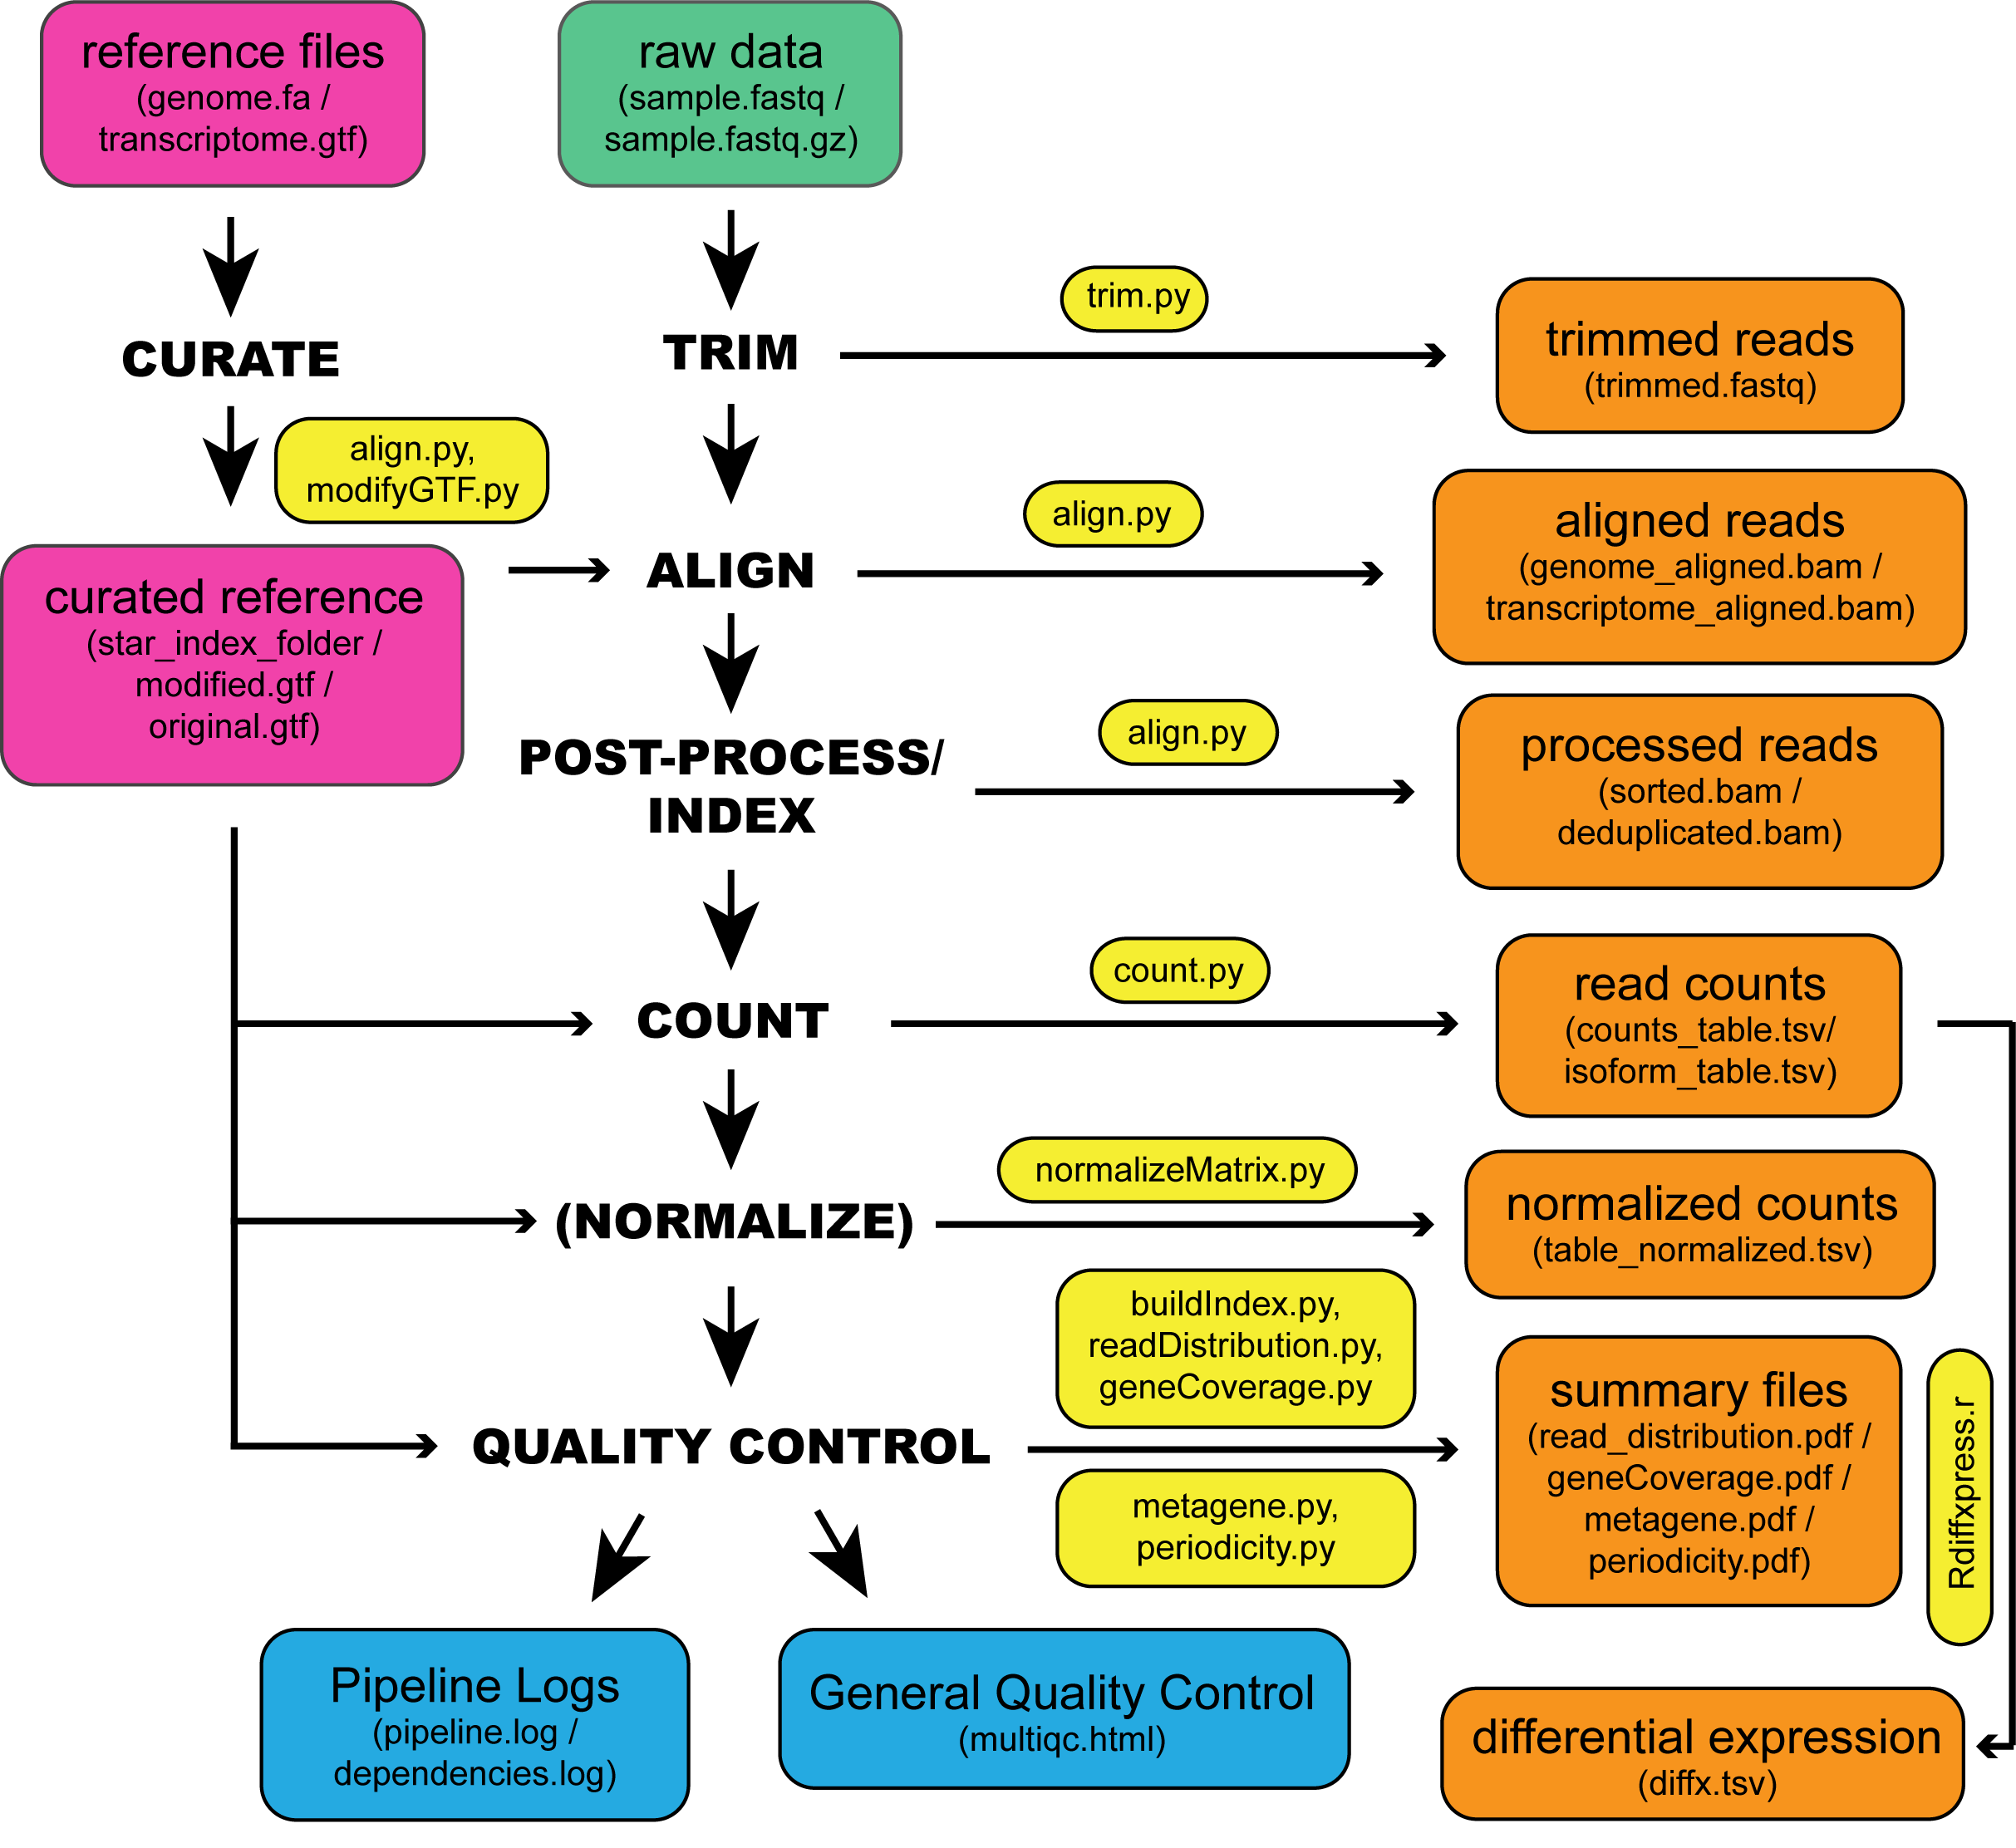
\includegraphics[width=80mm]{figures/xpresspipe_figure1.png}
  \caption{\textbf{An example schematic of the inputs required by XPRESSpipe and organization of the outputs.} Representation of the general steps performed by XPRESSpipe and data and log outputs. Steps in parentheses are optional to the user.}
  \label{fig:outputs}
\end{figure*}


\subsection*{Benchmarking Against Published Ribosome Profiling Data and New Insights}
The integrated stress response (ISR) is a signaling mechanism used by cells and organisms in response to a variety of cellular stresses \cite{harding_isr}. Although acute ISR activation is essential for cells to properly respond to stresses, long periods of sustained ISR activity can be damaging. These prolonged episodes contribute to a variety of diseases, including many that result in neurological decline \cite{isr_disease}. A recently discovered small-molecule inhibitor of the ISR, ISRIB, has been demonstrated to potentially be a safe and effective therapeutic for traumatic brain injury and other neurological diseases. Interestingly, ISRIB can suppress the damaging chronic low activation of the ISR, while it does not interfere with a cytoprotective acute, high-grade ISR. It has also been shown to be neuroprotective in mouse models of traumatic brain injury, adding to its wide pharmacological interest \cite{isrib_activation, isrib_structure, isrib_riboseq, isrib_neuroprotective, isrib_neuroprotective2, isrib_neuroprotective3, isrib_neuroprotective4}. \par

A recent study (data available under Gene Expression Omnibus accession number GSE65778) utilized ribosome profiling to better define the mechanisms of ISRIB action on the ISR, modeled by 1-hour tunicamycin (Tm) treatment in HEK293T cells \cite{isrib_riboseq}. A key finding of this study is that a specific subset of stress-related transcription factor mRNAs exhibit increased translational efficiency (TE) compared to untreated cells during the tunicamycin-induced ISR. However, when cells were co-treated with tunicamycin and ISRIB, the TE of these stress-related mRNAs showed no significant increase compared to untreated cells, which indicates that ISRIB can counteract the translational responses associated with the ISR. \par

To showcase the utility of XPRESSpipe in analyzing ribosome profiling and sequencing datasets, we re-processed and analyzed this dataset using the more current \textit{in silico} techniques included in the XPRESSpipe package to further query the translational mechanisms of the ISR and ISRIB. All XPRESSpipe-processed biological replicate samples exhibited a strong correlation between read counts per gene when thresholded similarly to count data available with the original publication (Spearman $\rho$ values 0.991-0.997) (Figure \ref{fig:figure2}A; Figure \ref{fig:supplement2}B shows the corresponding plots using the count data provided with the original publication for reference). \par

Compared to the raw count data made available in the original manuscript, when XPRESSpipe-processed samples were thresholded as in the original published raw count data, samples showed generally comparable read counts per gene between the two analytical regimes (Spearman $\rho$ values 0.937-0.950) (Figure \ref{fig:figure2}B). This is in spite of the fact that the methods section of the original publication employed software that was current at the time but is now outdated, such as TopHat2 \cite{tophat2}, which has a documented higher false positive alignment rate, generally lower recall, and lower precision at correctly aligning multi-mapping reads compared to STAR \cite{alignment_benchmark, star}. Many of the genes over-represented in the original count data as compared to data processed by XPRESSpipe are genes that have pseudogenes or other paralogs (Figure \ref{fig:supplement2}A highlights a sampling of some extreme cases). As these genes share high sequence similarity with each other, reads mapping to these regions are difficult to attribute to a specific genomic locus and are often excluded from further analyses due to their multi-mapping nature. The benchmarking study \cite{alignment_benchmark} that examined these and other aligners described how TopHat2 had a disproportionally high rate of incorrectly aligned bases, or bases that were aligned uniquely when they should have been aligned ambiguously, at least partially explaining the observed overcounted effect with TopHat2. Had TopHat2 marked problematic reads as ambiguous, they would have been excluded from later quantification. \par

Additionally, when TopHat2 and STAR were tested using multi-mapper simulated test data of varying complexity, TopHat2 consistently suffered in precision and recall. These calls are increasingly more difficult to make with smaller reads as well, and this is evident from Figure \ref{fig:figure2}B, where ribosome footprint samples consistently showed more over-counted genes than the corresponding RNA-Seq samples. When dealing with a ribosome footprint library of about 50-100 million reads, and with TopHat2's simulated likelihood of not marking an ambiguous read as such being about 0.5\% higher than STAR, this would lead to around 250,000 to 500,000 spuriously aligned reads, which is in line with our observations (all benchmarking details were derived from \cite{alignment_benchmark}). \par

An additional potential contributor to this divergence is that the alignment and quantification within XPRESSpipe use a current human transcriptome reference, which no doubt contains updates and modifications to annotated canonical transcripts and so forth when compared to the version used in the original study. However, in practice, these effects are modest for this dataset (Figure \ref{fig:supplement3}). While differences in processing between the outdated and current methods may not always create broad differences in output, key biological insights may be missed. The analysis that follows is exploratory and only meant to suggest putative targets identifiable by re-analyzing pre-existing, publicly available data. \par

\begin{figure*}
\centering
  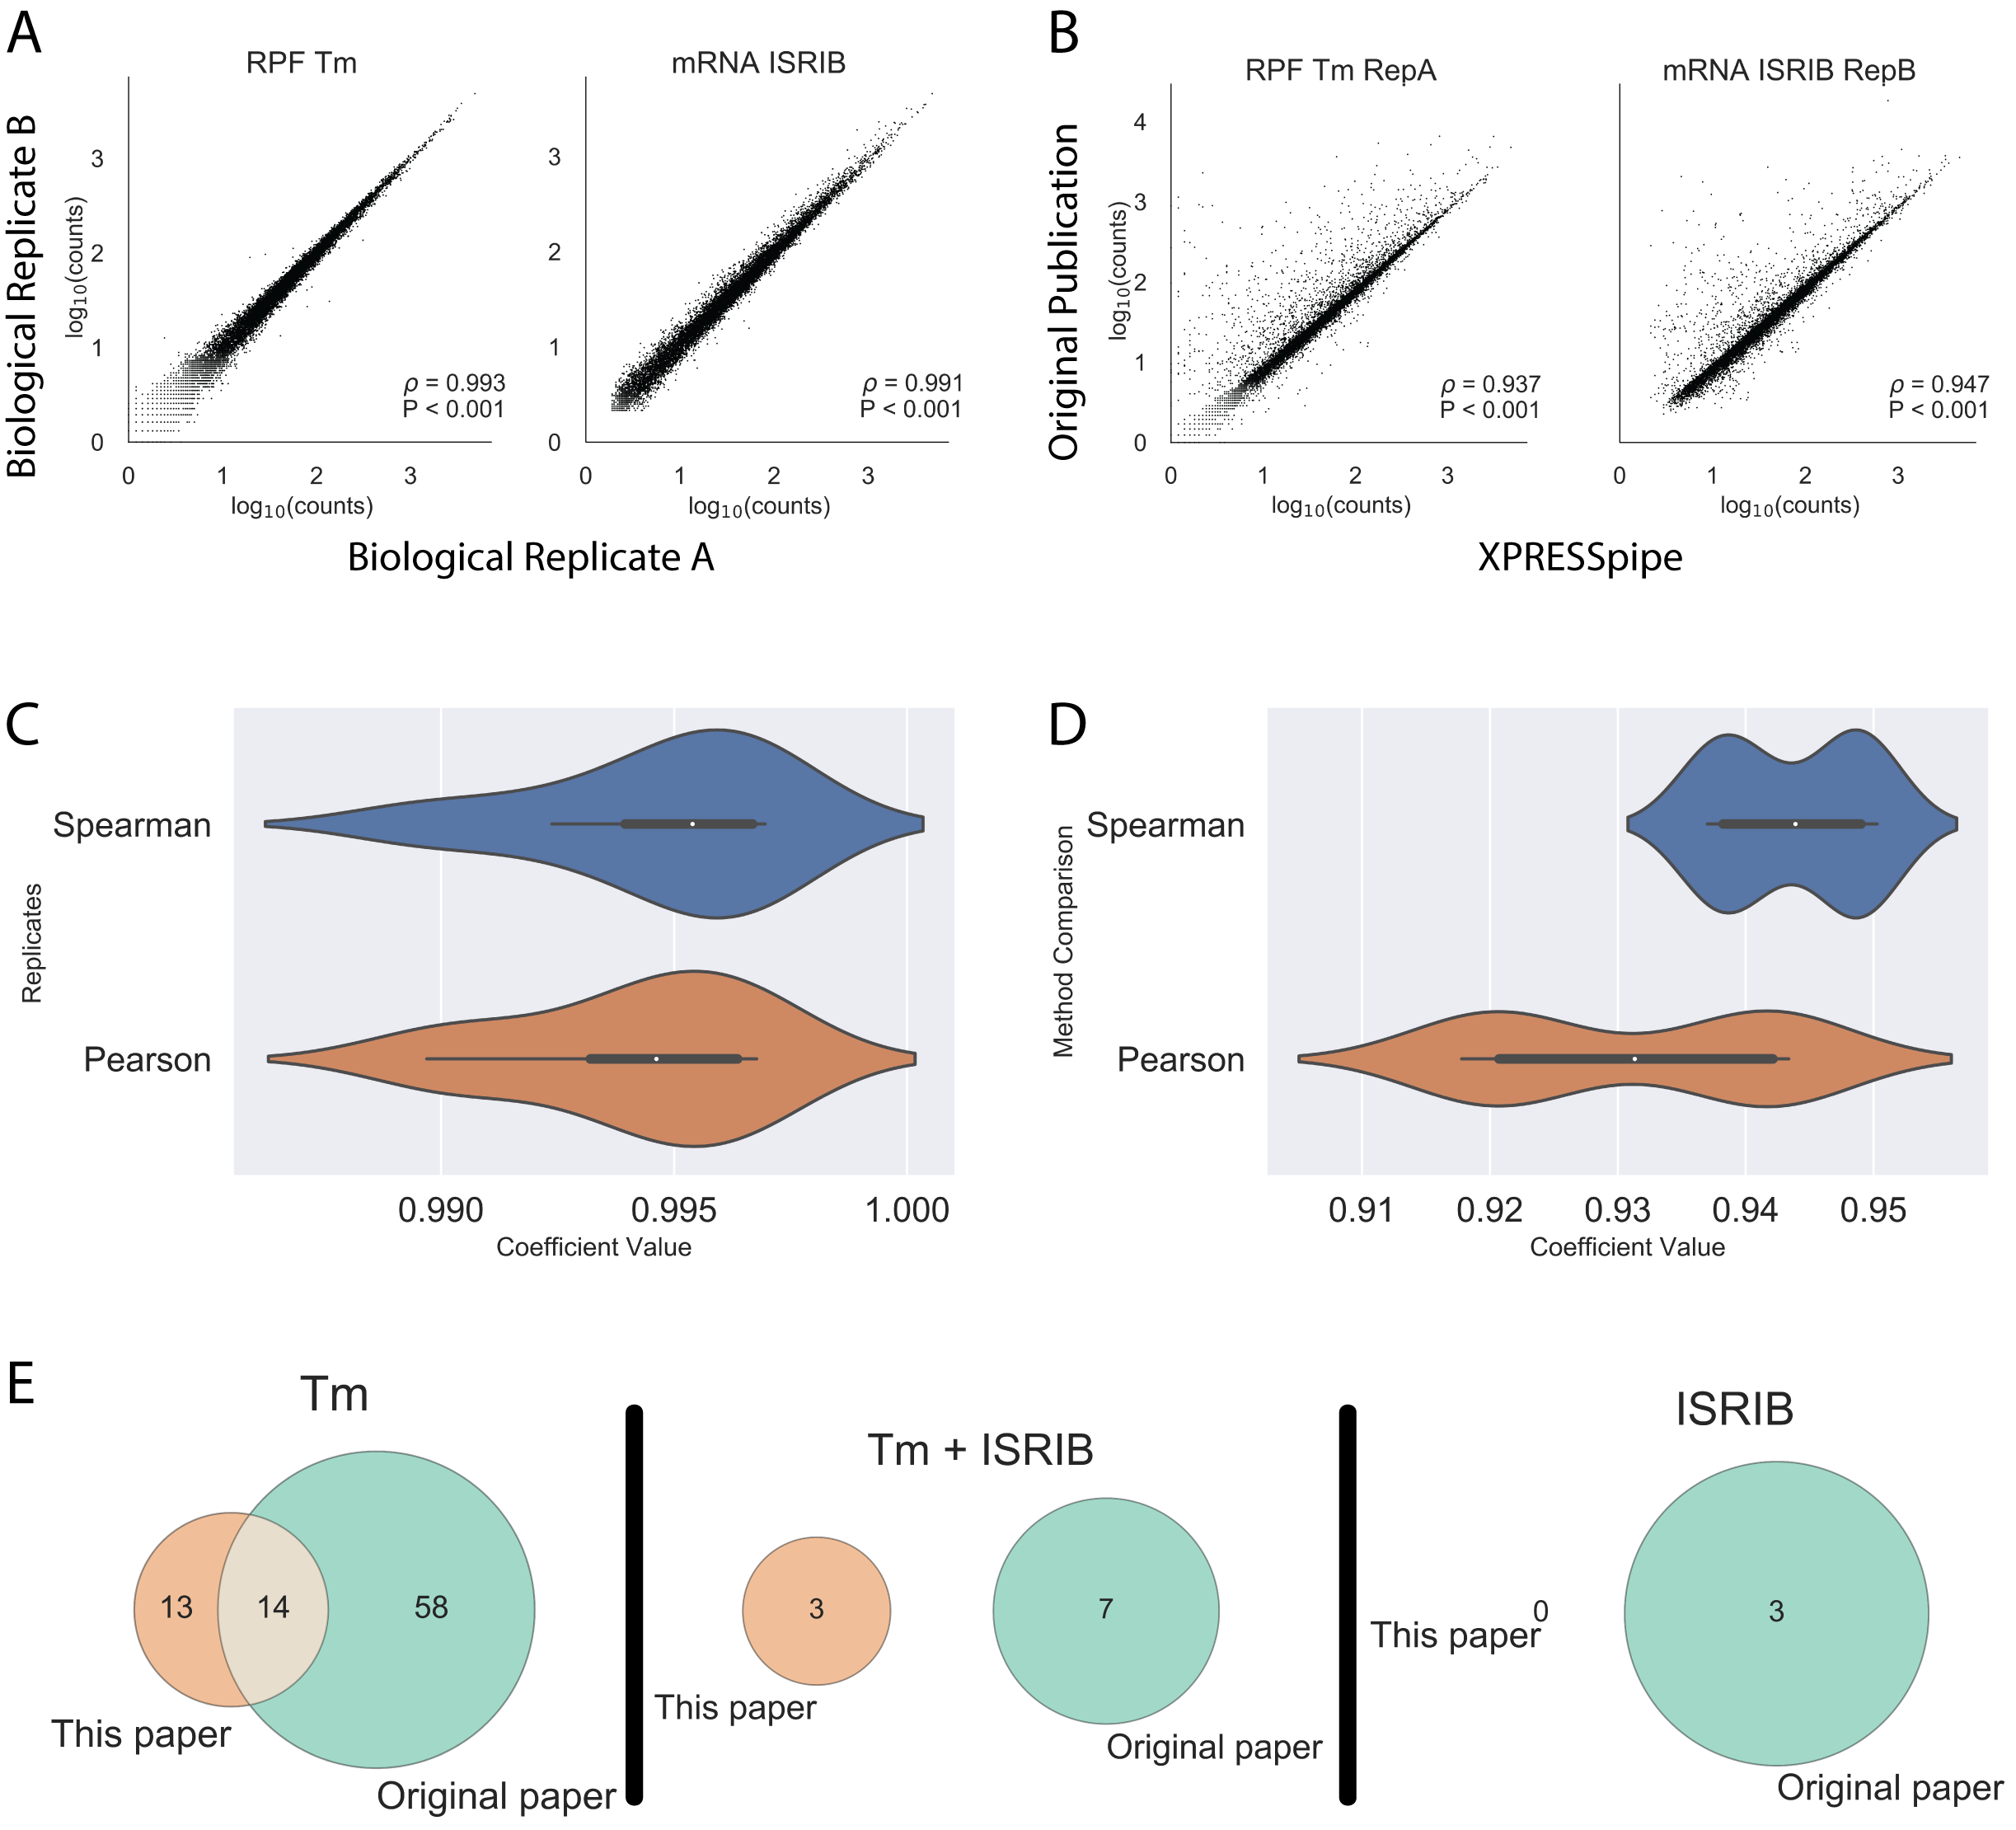
\includegraphics[width=145mm]{figures/xpresspipe_figure2.png}
  \caption{\textbf{Comparison between processed data produced by XPRESSpipe and original study.} Genes were eliminated from analysis if any RNA-Seq sample for that gene had fewer than 10 counts. A) Comparison of biological replicate read counts processed by XPRESSpipe. B) Comparison of read counts per gene between count data from the original study and the same raw data processed and quantified by XPRESSpipe. RPF, ribosome-protected fragments. Tm, tunicamycin. All $\rho$ values reported are Spearman correlation coefficients. XPRESSpipe-processed read alignments were quantified to \textit{Homo sapiens} build CRCh38v96 using a protein-coding only, truncated GTF.}
  \label{fig:figure2}
\end{figure*}

\begin{figure*}
\centering
  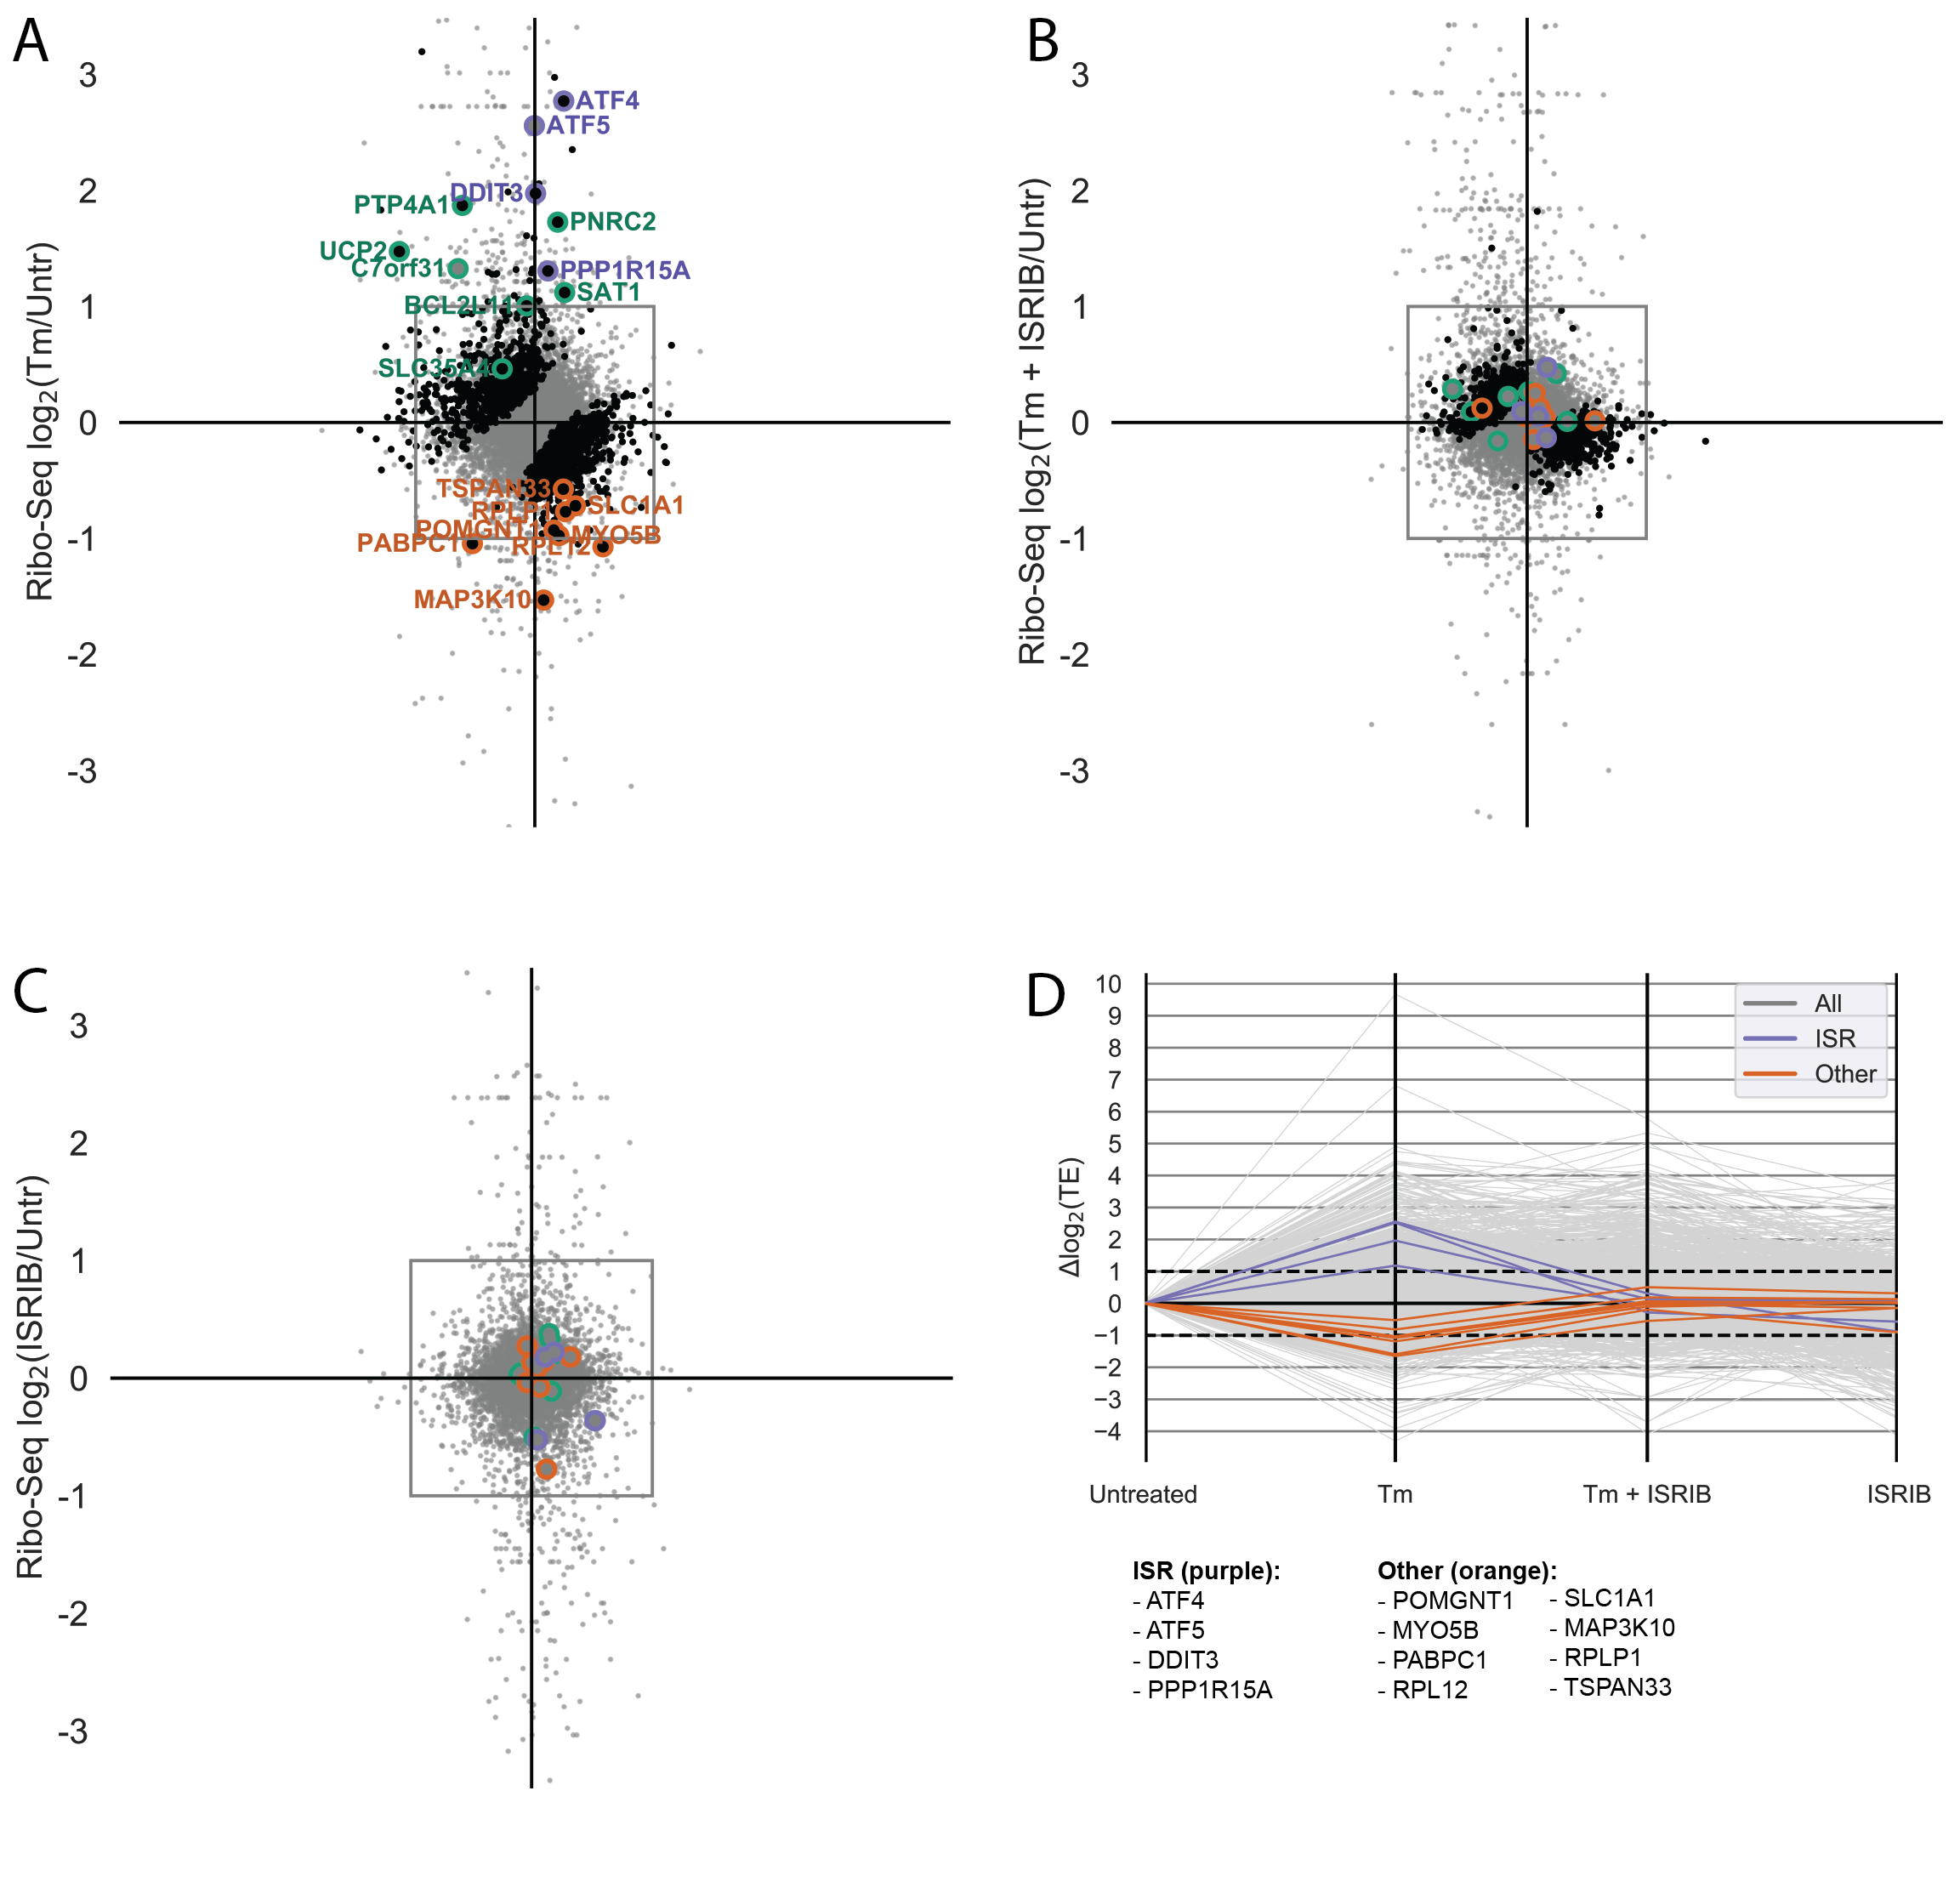
\includegraphics[width=180mm]{figures/xpresspipe_figure3.png}
  \caption{\textbf{Analysis of previously published ISR TE data using XPRESSpipe.} A-C) Log\textsubscript{2}(Fold Change) for each drug condition compared to untreated for the ribosome profiling and RNA-Seq data. Purple, ISR canonical targets highlighted in the original study. Green, genes with uORFs affected by ISR as highlighted in the original study. Orange, genes fitting a strict thresholding paradigm to identify genes that display a 2-fold or greater increase in TE in Tm + ISRIB treatment compared to Tm treatment. Black, genes with statistically significant changes in TE. Grey, all genes. Changes in ribo-seq and mRNA-Seq were calculated using DESeq2. TE was calculated using DESeq2. Points falling outside of the plotted range are not included. D) Changes in log\textsubscript{2}(TE) for each drug condition compared to untreated control. Grey, all genes. Purple, ISR targets identified in the original study. Orange, genes fitting a strict thresholding paradigm to identify genes that display a 2-fold or greater increase in TE in Tm + ISRIB treatment compared to Tm treatment. XPRESSpipe-processed read alignments were quantified to \textit{Homo sapiens} build CRCh38v96 using a protein-coding only, truncated GTF.}
  \label{fig:figure3}
\end{figure*}

Similar canonical targets of translation regulation during ISR were identified in the XPRESSpipe-processed data as were identified in the original study. These targets include ATF4, ATF5, PPP1R15A, and DDIT3 (Figure \ref{fig:figure3}A-C, highlighted in purple) \cite{isrib_riboseq}. Of note, the fold-change in ribosome occupancy of ATF4 (6.83) from XPRESSpipe-processed samples closely mirrored the estimate from the original publication (6.44). Other targets highlighted in the original study \cite{isrib_riboseq}, such as ATF5, PPP1R15A, and DDIT3 also demonstrated comparable increases in their ribosome occupancy fold-changes to the original publication count data (XPRESSpipe: 5.89, 2.47, and 3.93; respectively. Original: 7.50, 2.70, and 3.89; respectively) (Figure \ref{fig:figure3}A). Similar to the originally processed data, all of these notable changes in ribosome occupancy return to untreated levels during Tm + ISRIB co-treatment (Figure \ref{fig:figure3}B). Additional ISR targets containing micro-ORFs described in the study (highlighted in green in Figure \ref{fig:figure3}A-C) were also similar in translational and transcriptional regulation across conditions between the two analyses. \par

Both the original study and our XPRESSpipe-based re-analysis show that ISRIB can counteract the significant increase in TE for a set of genes during ISR. To further explore TE regulation during ISR, we asked if ISRIB has a similar muting effect on genes with significant decreases in TE induced by the ISR. In the original study, genes with significant decreases in TE were reported in a source-data table but not a focus in the study. However, re-analysis of these data with the updated XPRESSpipe methodology identifies genes whose translational down-regulation may play a role in the neurodegenerative effects of ISR and the neuroprotective properties of ISRIB \cite{isrib_neuroprotective,isrib_neuroprotective2,isrib_neuroprotective3,isrib_neuroprotective4}. Importantly, several of these genes were not identified as having significantly down-regulated TEs in the original analysis, which suggests why a focus on translational downregulation may have been foregone. In all, we identified eight genes with the regulatory paradigm of interest: significant decreases in TE during tunicamycin-induced ISR that are rescued in the ISR + ISRIB condition (Table \ref{tab:targets}, descriptions sourced from \cite{genecards, ncbi, uniprot} (Figure \ref{fig:figure3}D). RNA-Seq and ribosome-footprint coverage across these genes show that the significant changes in their TE are due to neither spurious, high-abundance fragments differentially present across libraries nor variance from an especially small number of mapped reads (Figure \ref{fig:supplement4}). This is an important consideration as the commonly suggested use of the CircLigase enzyme in published ribosome profiling library preparation protocols, which circularizes template cDNA before sequencing, can bias certain molecules' incorporation into sequencing libraries based on read-end base content alone \cite{circligase_bias}. \par

Four (POMGNT1, SLC1A1, MAP3K10, TSPAN33) out of the eight identified genes have annotated neurological functions or are integrally tied to a pathway that functions in neurogenesis, which suggests their regulation may be functionally important for the neurodegenerative effects of ISR and the neuroprotective properties of ISRIB. For example, SLC1A1 is a glutamate transporter expressed throughout the brain where it plays vital roles in neurotransmission and extracellular glutamate homeostasis. Glutamate transporters, like SLC1A1, have also been implicated in preventing neurotrauma within the first few minutes of insult, and deficits in this transporter can lead to neurotoxic levels of glutamate \cite{slc1a1_neurotoxic}. Finally, down-regulation of SLC1A1 has already been implicated in diseases such as neurodegenerative diseases caused by mutations in the eukaryotic translation initiation factor 2B subunit epsilon (eIF2B5) that mimic the effects of phosphorylated eIF2$\alpha$ on cellular stress response and translation \cite{eif2b_neuroprotective, isrib_riboseq, isrib_structure}. This suggests that TE regulation of SLC1A1 abundance by translation initiation factors might be important in the neurodegeneration observed in prolonged ISR conditions. ISRIB's neuroprotective effects may, therefore, stem from a recovery of SLC1A1 protein expression to wild-type levels, which in turn helps restore normal glutamate regulation. Though speculative, these ISRIB-responsive neuronal targets act as interesting cases for further validation and study in a model more representative of neurotoxic injury and disease than the HEK-293T model used in the original study. In all, this comparison demonstrates the utility of XPRESSpipe for rapid, user-friendly analysis and re-analysis of ribosome-profiling experiments in the pursuit of biological insights and hypothesis generation. \par

\begin{table*}[!]
    \centering
\captionof{table}{\textbf{Translationally down-regulated genes during acute Tm treatment and recovered regulation during Tm + ISRIB treatment.} Gene names with an asterisk indicate these genes were identified as significantly down-regulated during Tm treatment in the original manuscript.}
\begin{tabular}{p{2.5cm}p{15.5cm}}
 \textbf{Gene Name} & \textbf{Relevant Description} \\
 \hline
 POMGNT1 & Participates in O-mannosyl glycosylation. Mutations have been associated with muscle-eye-brain diseases and congenital muscular dystrophies. Expressed especially in astrocytes, as well as in immature and mature neurons. Expressed across brain stem cells. \\
 \hline
 MYO5B* & May be involved in plasma membrane recycling. No related neurological annotations. \\
 \hline
 PABPC1 & Binds the poly(A) tail of mRNA. Promotes ribosome recruitment and translation initiation. May contribute to mRNA stability. No related neurological annotations. \\
 \hline
 RPL12 & Ribosomal subunit. No related neurological annotations. \\
 \hline
 SLC1A1 & Dense expression in substantia nigra, red nucleus, hippocampus, and cerebral cortical layers. Member of high-affinity glutamate transporter. In the brain, crucial for terminating postsynaptic action of the neurotransmitter glutamate. Responsible for maintaining glutamate concentrations below neurotoxic levels. \\
 \hline
 MAP3K10* & Functions in JNK signaling, reportedly involved in nerve growth factor induces neuronal apoptosis. Expressed in the cerebral cortex. Activates NEUROD1, which promotes neuronal differentiation. \\
 \hline
 RPLP1 & Ribosome subunit. Evidence for stem cell and embryonic expression in the cerebral cortex. \\
 \hline
 TSPAN33 & Plays a role in normal erythropoiesis and regulates maturation and trafficking of ADAM10, a metalloprotease. Negatively regulates Notch activity by way of its regulation of ADAM10. Notch signaling is vital to neurogenesis. \\
 \label{tab:targets}
\end{tabular}
\end{table*}


\subsection*{Benchmarking Against TCGA Data}
To further validate the design, reliability, and versatility of the XPRESSpipe pipeline, we processed raw TCGA sequence data using XPRESSpipe and compared the output count values to those publicly available through TCGA \cite{tcga}. Spearman $\rho$ values for the selected samples ranged from 0.984-0.986 (Figure \ref{fig:figure4}), indicating XPRESSpipe performs with similar accuracy to the TCGA RNA-Seq processing standards. \par

The differences in reported counts can be accounted for by a couple of key differences. For instance, the XPRESSpipe-processed files are aligned to the \textit{Homo sapiens} GRChv96 reference transcriptome, while the original count data are aligned to the GRChv79 reference transcriptome. The use of a different transcriptome reference can result in variance in the final quantified data for several genes (Figure \ref{fig:supplement5}). For example, in the four years between these versions, significant advances have been made in our understanding of transcribed regions of the human genome. Between versions 95 and 96 alone (version 95 published 24 Nov 2018, version 96 published 13 Mar 2019), at least 32,259 records were added (quantified simply by the difference in line numbers between the files, although in addition other records have been removed or modified). \par

Another source of dissimilarity in data processing appears to arise if an Ensembl canonical transcripts-only reference is used during quantification. TCGA-processed data used an un-modified transcriptome reference file (all transcripts); therefore, the use of this modified (Ensembl canonical transcripts only) GTF will produce varied quantification for some genes as quantifications are constrained to a single transcript version of a given gene and a read will not be quantified if mapping to an exon not used by the canonical transcript. Even using XPRESSpipe settings closest to the TCGA pipeline and using the same genome and transcriptome version resulted in some variation (Figure \ref{fig:supplement5}, plot enclosed in maroon). By performing a more detailed analysis of these differences, it is clear that virtually all genes exhibiting variance between the processing methods are pseudogenes, with the TCGA pipeline accepting and quantifying more pseudogenes at the time of initial analysis of this dataset. This can be indicative of the difficulty surrounding the recognition of these reads as multi-mapping to both the original gene and pseudogene (Figure \ref{fig:supplement6}, \ref{fig:supplement7}, \ref{fig:supplement8}; interactive plots accompanying Figure \ref{fig:supplement8} can be accessed at \cite{manuscript}. \par


\begin{figure*}
\centering
  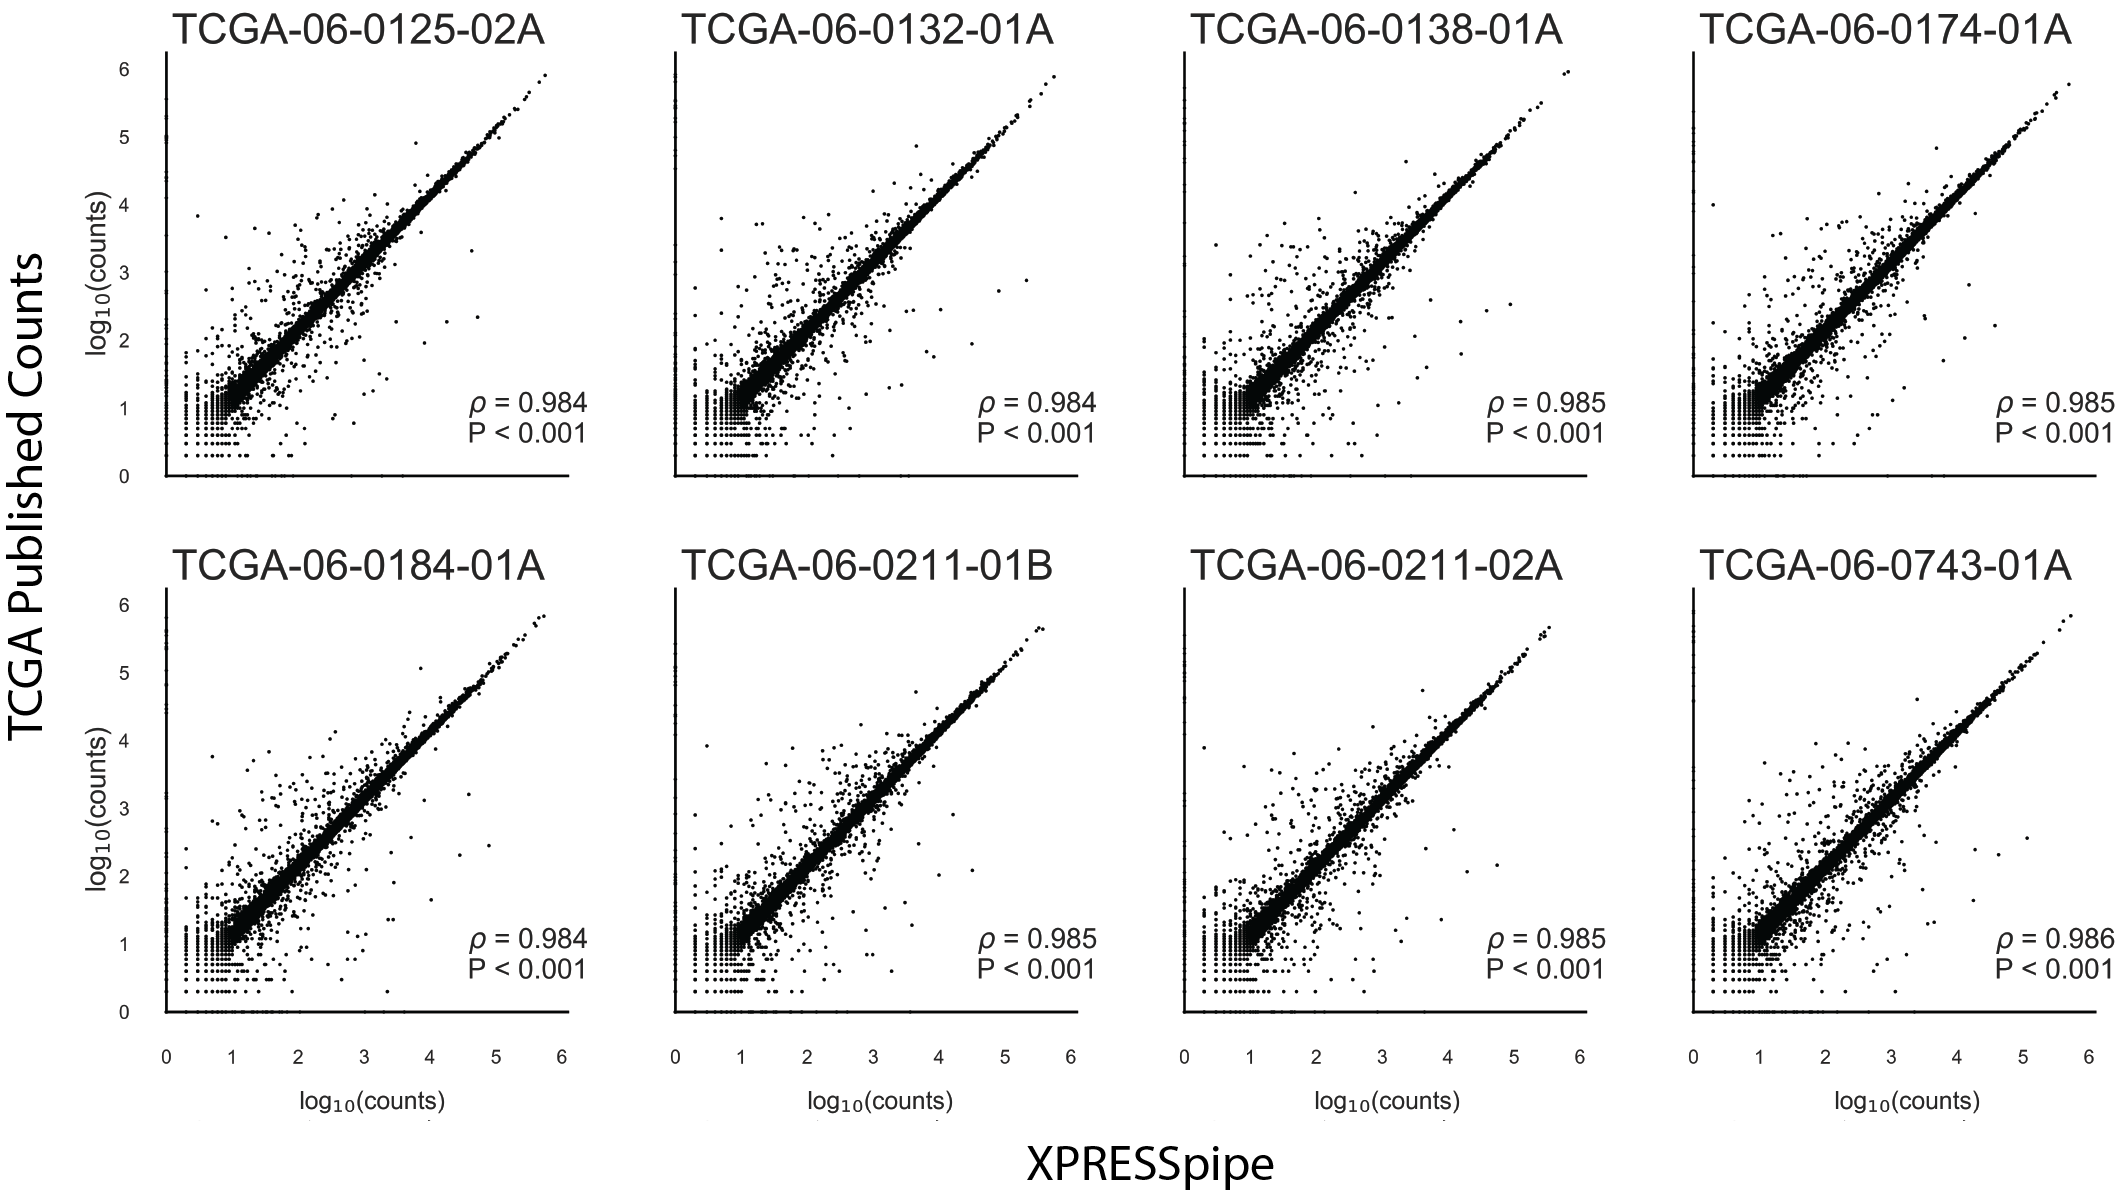
\includegraphics[width=180mm]{figures/xpresspipe_figure4.png}
  \caption{\textbf{Pipeline validation using publicly available TCGA count data.} Correlations were calculated between publicly available count data from TCGA samples and the count data processed by XPRESSpipe. Pseudogenes were excluded from the analysis. All reported $\rho$ values are Spearman correlation coefficients. XPRESSpipe-processed read alignments were quantified to \textit{Homo sapiens} build CRCh38v96 using an unmodified GTF.}
  \label{fig:figure4}
\end{figure*}


\subsection*{Cost Analysis}
XPRESSpipe functions can be computationally intensive, and thus, super-computing resources are recommended, especially when handling large datasets or when aligning to larger, more complex genomes, such as \textit{Homo sapiens}. Many universities provide super-computing resources to their affiliates; however, in cases where these resources are not available, servers such as Amazon Web Services (AWS) \cite{aws} can be used to process sequencing data using XPRESSpipe. Table \ref{tab:chpc_performance} outlines runtime statistics for the ISRIB dataset used in this study. As a general estimate, this amounts to about 40 minutes per incoming FASTQ file, including copying each file into the cluster filesystem (about 8 GB per file in this example) and performing all quality control analyses after read processing. This will certainly vary depending on the number of files input, the steps being performed, and so forth. The ISRIB ribosome profiling dataset contained a total of 32 raw sequence files that were align to \textit{Homo sapiens}, thus it acts as a high-end estimate of the time required to process data with XPRESSpipe. \par

\begin{table*}[!]
    \centering
\captionof{table}{\textbf{XPRESSpipe processing statistics for dataset GSE65778.}}
\begin{tabular}{p{5cm}p{3cm}}
\textbf{Metric} & \textbf{Value} \\
 \hline
 Total Raw Input & 257 GB \\
 \hline
 Total Output & 500 GB \\
 \hline
 Elapsed Real Time & 22h 18m \\
 \hline
 Allocated CPUs & 16 \\
 \hline
 Allocated Memory per Node & 64GB \\
 \label{tab:chpc_performance}
\end{tabular}
\end{table*}

Processing a sequencing dataset like this could be performed on a platform such as AWS relatively inexpensively. For a comparable dataset, cost to use a computational node with similar specifications for the above elapsed time would be approximately 17.13 USD using an Amazon EC2 On-Demand m5.4xlarge node (however, significantly reduced rates are available if using Spot instances or by using the free tier) and storage cost would amount to around 11.5 USD/month on Amazon S3 storage. In most cases, the user might only be interested in keeping the final quantified data (i.e., gene counts tables) and quality control analyses and metrics which are relatively small in size and could thus be stored locally long-term, removing the need for S3 or other cloud storage options of intermediate files. However, it is essential users store their raw sequence files long-term, or host them on a public database, such as the Gene Expression Omnibus (GEO). \par


\section*{Discussion}
We have described a new software suite, XPRESSyourself, which includes a set of tools to aid in the processing and analysis of expression data, and other applications of RNA-Seq such as ribosome profiling. Although RNA-Seq technologies are quite advanced, standardized computational protocols are much less established for some applications. This is problematic when individuals or groups may not be using the most up-to-date methods or may not be aware of particular biases or measures of quality control required to produce a reliable, high-quality sequencing study. XPRESSpipe handles these issues through on-going curation of benchmarked software tools and by simplifying the required user input. It also outputs all necessary quality control metrics so that the user can quickly assess the quality of their data and identify any systematic problems or technical biases that may compromise their analysis. \par

One particular benefit of XPRESSyourself is that it consolidates, streamlines, and/or introduces many tools specific to ribosome profiling processing and analysis. This includes producing GTF files with $5'$- and $3'$- truncated CDS annotations, rRNA probe design for subtractive hybridization of abundant rRNA contaminants, and automated quality-control analyses to report on ribosome footprint periodicity and metagene coverage. These tools will help to democratize aspects of ribosome profiling for which software have not been previously publicly available. \par

An additional problem XPRESSpipe addresses is the incorrect use of these software tools, which is especially important for those coming from a non-computational background, but often applies to experienced users who simply cannot keep up with the plethora of advances and benchmarking in the field. XPRESSyourself will remove this barrier-to-entry for most users so that they can process and analyze their data immediately upon receipt of the raw data and only requires simple programming knowledge that is included in video walkthroughs, example scripts, and interactive command builders within this software suite. \par

We demonstrated the utility of the XPRESSyourself toolkit by re-analyzing a publicly available ribosome profiling dataset. From this analysis, we identified putative translational regulatory targets of the integrated stress response (ISR) that may contribute to its neurodegenerative effects and their rescue by the small-molecule ISR inhibitor, ISRIB. This highlights the importance of re-analyzing published datasets with more current methods, as improved analysis methodologies and updated organism genome references may result in new interpretations and hypotheses. \par

XPRESSyourself will enable individuals and labs to process and analyze their own data, which will result in quicker turnaround times of experiments and financial savings. XPRESSyourself will also put missing or incomplete computational tools required for ribosome profiling and RNA-Seq into the hands of the user. Additionally, the inclusion of detailed log reports, summaries of software dependencies used during runtime, and containerized versions of the pipeline where dependencies are archived and self-contained will aid in reproducibility and make transparent methods easy to incorporate into the resulting publications. \par


\section*{Conclusions}
With the adoption of this flexible pipeline, the field of high-throughput sequencing, particularly ribosome profiling, can continue to standardize the processing protocol for associated sequence data and eliminate the variability that comes from the availability of a variety of software packages for various steps during sequence read processing. Additionally, XPRESSpipe consolidates various tools used by the ribosome profiling and RNA-Seq communities. With these tools, genome reference formatting and curation is automated and accessible to the public. Other tools, like those for GTF CDS truncation, rRNA depletion, and intron-less gene coverage plotting, are introduced within this software suite to enhance the current RNA-Seq toolkit. Further, by using this pipeline on publicly available data, we highlight the utility of XPRESSpipe to process publicly available or personal data to uncover novel biological patterns quickly. Adoption of this tool will allow scientists to quickly process and access their data independently, guide them in understanding key considerations in processing their data, and standardize protocols for applications of RNA-Seq, thus increasing the reproducibility of sequencing analyses.


\section*{Materials and Methods}
Methods described in this manuscript apply to the software packages at the time of writing. To obtain the most current methods, please refer to the documentation or source code for a given module.

\subsection*{Software Dependencies}
A list of dependencies required for XPRESSpipe at the time of writing is listed in Table \ref{Tab:software_pipe}. Dependencies for XPRESSplot at the time of writing are listed in Table \ref{Tab:software_plot}.

% Software dependencies table
\begin{table*}[!]
    \centering
\captionof{table}{\textbf{Summary of dependency software, accession location, and purpose in the XPRESSpipe package.}}
\begin{tabular}{p{3cm}p{7.5cm}p{2.4cm}}
 \textbf{Package} & \textbf{Purpose} & \textbf{Reference} \\
 \hline
 Python & Primary language & \\
 \hline
 R & Language used for some statistical modules & \\
 \hline
 fastp & Read pre-processing & \cite{fastp} \\
 \hline
 STAR & Reference curation and read alignment & \cite{star} \\
 \hline
 samtools & Alignment file manipulation & \cite{samtools} \\
 \hline
 bedtools & Alignment file manipulation & \cite{bedtools} \\
 \hline
 Cufflinks & Read quantification (primary) & \cite{cufflinks} \\
 \hline
 HTSeq & Read quantification & \cite{htseq} \\
 \hline
 FastQC & Quality Control & \cite{fastqc} \\
 \hline
 MultiQC & Quality Control & \cite{multiqc} \\
 \hline
 Pandas & Data manipulation & \cite{pandas} \\
 \hline
 NumPy & Data manipulation & \cite{numpy1, numpy2} \\
 \hline
 SciPy & Data manipulation & \cite{scipy} \\
 \hline
 scikit-learn & Data manipulation & \cite{sklearn} \\
 \hline
 Matplotlib & Plotting & \cite{matplotlib} \\
 \hline
 XPRESSplot & Normalization and matrix manipulation & This paper \\
 \hline
 GenomicAlignments & BAM file processing & \cite{genomicalign} \\
 \hline
 GenomicFeatures & GTF file processing & \cite{genomicalign} \\
 \hline
 dupRadar & Perform library complexity calculations & \cite{dupradar} \\
 \hline
 riboWaltz & Perform p-site offset calculations & \cite{ribowaltz} \\
 \hline
 DESeq2 & Perform differential expression analysis & \cite{deseq2} \\
 \label{Tab:software_pipe}
\end{tabular}
\end{table*}

% Software dependencies table
\begin{table*}[!]
    \centering
\captionof{table}{\textbf{Summary of dependency software, accession location, and purpose in the XPRESSplot package.}}
\begin{tabular}{p{2.4cm}p{7.5cm}p{3cm}}
 \textbf{Package} & \textbf{Purpose} & \textbf{Reference} \\
 \hline
 Python & Primary language & \\
 \hline
 R & Language used for some statistical modules & \\
 \hline
 Pandas & Data manipulation & \cite{pandas} \\
 \hline
 NumPy & Data manipulation & \cite{numpy1, numpy2} \\
 \hline
 SciPy & Data manipulation & \cite{scipy} \\
 \hline
 Matplotlib & Plotting & \cite{matplotlib} \\
 \hline
 Seaborn & Plotting & \cite{seaborn} \\
 \hline
 Plotly & Interactive plotting & \cite{plotly} \\
 \hline
 scikit-learn & Data manipulation & \cite{sklearn} \\
 \hline
 SVA & Perform batch correction for known effects & \cite{sva} \\
 \label{Tab:software_plot}
 \end{tabular}
\end{table*}

\subsection*{Installation}
XPRESSyourself software packages are hosted at https://github.com/XPRESSyourself. Current or past versions of XPRESSyourself packages can be found at their respective repositories under the XPRESSyourself project. For simplest installation, we recommend using the Anaconda package manager \cite{anaconda}. Using the method below, you will need to activate the environment every time you wish to use XPRESSyourself software. Download XPRESSpipe's source code, set up the Anaconda environment, and install XPRESSpipe and XPRESSplot, as below (providing the version number you would like to download):

\begin{lstlisting}[language=bash, caption=XPRESSyourself installation]
$ curl -L -O https://github.com/XPRESSyourself/\
              XPRESSpipe/archive/v0.2.1b0.tar.gz
$ tar xvzf v0.0.0.tar.gz
$ cd XPRESSpipe-0.0.0
$ conda env create --name xpresspipe -f \
                          requirements.yml
$ conda activate xpresspipe
$ python setup.py install
\end{lstlisting}

\subsection*{Running XPRESSpipe}
Before processing data, the appropriate reference files must be curated. Download the FASTA and GTF files for the organism of interest, change the GTF file name to \texttt{transcripts.gtf}, and run the code below. This will generate the appropriate STAR index files, as well as a GTF file with protein-coding transcripts only and the $5'$- and $3'$- end of each transcript truncated for ribosome profiling data. More examples of how to curate reference files can be found in the documentation \cite{xpresspipe_docs}.

\begin{lstlisting}[language=bash, caption=curateReference example]
$ xpresspipe curateReference \
             -o /path/to/reference/ \
             -f /path/to/reference/fasta_genome/ \
             -g /path/to/reference/transcripts.gtf \
             --protein_coding \
             --truncate \
             --truncate_5prime 45 \
             --truncate_3prime 15 \
             --sjdbOverhang 49 \
             --max_processors None
\end{lstlisting}

To process data, a simplistic example is provided below, but additional parameter changes may be necessary. Refer to the help menu (\texttt{xpresspipe --help}) or the documentation \cite{xpresspipe_docs} for more information and examples of how to tune these parameters.

\begin{lstlisting}[language=bash, caption=riboseq pipeline example]
$ xpresspipe riboseq \
              -i /path/to/input_dir \
              -o /path/to/output_dir \
              -r /path/to/curated_reference \
              --gtf /path/to/transcripts_CT.gtf \
              -e isrib_dataset \
              -a CTGTAGGCACCATCAAT \
              --sjdbOverhang 49
\end{lstlisting}

Further analyses, such as additional gene coverage profiles, differential expression analysis, and batch normalization, can be performed. Details on how to perform these steps can be accessed from the help menu (\texttt{xpresspipe --help}) or the documentation \cite{xpresspipe_docs}.

\subsection*{Running XPRESSplot}
Installation is handled during install of XPRESSpipe, but if usage XPRESSplot alone is desired, the user can run:

\begin{lstlisting}[language=bash, caption=XPRESSplot install]
$ pip install xpressplot
\end{lstlisting}

Generally, two inputs are required for all functions within XPRESSplot:

\begin{enumerate}
  \item \textbf{Expression Matrix}: It is assumed that the input data matrix = \textit{i} * \textit{j} where \textit{i} (rows) are genes or other analytes and \textit{j} (columns) are samples.
  \item \textbf{Metadata Table}: It is assumed that the metadata table is a two-column, header-less data matrix where column 0 is the sample ID (as specified in \textit{j} column names of the expression matrix) and column 1 is the sample group (for example, genotype or treatment group).
\end{enumerate}

Usage of all xpressplot functionalities can be found in the documentation \cite{xpressplot_docs}.

\subsection*{GTF Modification}
To parallelize GTF modification, a GTF file is split into approximately proportional chunks equal to the specified number of threads. To avoid an incomplete gene record being included in a chunk and being inappropriately processed, a given chunk endpoint is determined by calculating the size of the GTF, dividing by the number of threads, and advancing to that endpoint, then advancing line by line until the last line of the gene record encountered at the endpoint. This is performed for each subsequent chunk. If creating the last chunk, the end of the chunk is the last line of the GTF record. \par

Ensembl canonical transcripts are determined according to the Ensembl glossary definition of a canonical transcript \cite{ensembl_canon}. For cases where a tie exists between equal priority transcripts, the longest is chosen. When there are multiple transcripts that tie for equal priority and longest length, the first listed record is retained. Exon or CDS lengths are calculated by taking the sum of each exon or CDS, not including intron or other space in the calculation. \par

Protein-coding records are retained by performing a simple string search for the ``protein\_coding" annotation in the attribute column of a GTF file. \par

Truncation of records is performed by identifying the $5'$- and $3'$- end of each transcript and modifying the given coordinates to reflect the given truncation amounts. Suggested truncation amounts are 45 nt from the $5'$- end and 15 nt from the $3'$- end, both of which are set as the default truncation amount parameters for the function and do not need to be modified unless the user desires \cite{ingolia_meth}. As a given CDS portion of a given exon may be less than a truncation amount, the function will perform a strand-aware recursive search CDS by CDS per transcript until the full truncation amount has been fully removed for each end. Any record smaller than the sum of the $5'$- and $3'$- truncation amounts is removed entirely from the output file. \par

\subsection*{Flattened GTF Records}
Flattened transcriptome references are created via a modified version of the annotation curation module available in riboWaltz \cite{ribowaltz}. Vectorized expressions in Pandas \cite{pandas} are performed to quickly parse out pertinent meta-information for each transcript for the given analysis. Intermediate files are created for retrieval by each process when parallelizing analysis of each alignment file. This allows for fast processing of each BAM file, where the bottleneck in speed arises from the decompression and import of the binary alignment data. Flat files are automatically destroyed after sub-module completion. \par

\subsection*{Normalization}
Equations 1-4 reflect the design of the normalization functions within XPRESSplot, where \textit{g} is gene \textit{n}, \textit{ge} is cumulative exon space for gene \textit{n}, \textit{r} is total reads, \textit{f} is total fragments, and \textit{l} is length.

  \begin{equation}
    RPM\textsubscript{g} = \frac{1e6 \cdot r\textsubscript{\textit{ge}}}{\sum_{g=1}^{n} r\textsubscript{\textit{ge}}}
  \end{equation}
  \begin{equation}
    RPKM\textsubscript{g} = \frac{1e9 \cdot r\textsubscript{\textit{ge}}}{(\sum_{g=1}^{n} r\textsubscript{\textit{ge}}) \cdot \textit{l} \textsubscript{\textit{ge}}}
  \end{equation}
  \begin{equation}
    FPKM\textsubscript{g} = \frac{1e9 \cdot f\textsubscript{\textit{ge}}}{(\sum_{g=1}^{n} f\textsubscript{\textit{ge}}) \cdot \textit{l} \textsubscript{\textit{ge}}}
  \end{equation}
  \begin{equation}
    TPM\textsubscript{g} = \frac{1e6 \cdot r\textsubscript{\textit{ge}}}{(\sum_{g=1}^{n} (\frac{1e3 \cdot r\textsubscript{\textit{ge}}}{l\textsubscript{\textit{ge}}})) \cdot \textit{l} \textsubscript{\textit{ge}}}
  \end{equation}


\subsection*{Quality Control Summary Plotting}
Summary plots are created using Pandas \cite{pandas} and Matplotlib \cite{matplotlib}. Kernel density plots for library complexity analyses are created using NumPy \cite{numpy1, numpy2} and SciPy's \texttt{gaussian\_kde} function \cite{scipy}.

\subsection*{Metagene Estimation}
Metagene calculations are performed by determining the meta-transcript coordinate \textit{M} for each read alignment within a transcriptome-aligned BAM file (automatically output by STAR within XPRESSpipe). Let \textit{L\textsubscript{e}} be the first mapped position of the read (strand agnostic and in reference to exon space to the $5'$-end) and \textit{r} be the length of the mapped read. Let \textit{$\ell$\textsubscript{e}} be the cumulative length of all exons for the given transcript. The subscripted \textit{e} indicates the coordinate is relative to the exon space (intronic ranges within a transcript do not contribute to total space calculation). Extreme outliers (i.e., top and bottom 0.5\% of transcripts ordered by their read abundances) are removed from analysis as they will inappropriately skew the meta-profile for the majority (99\%) of transcripts. Required inputs are a transcriptome-aligned BAM file and a GTF reference file, which is flattened for downstream processing. For each mapped coordinate, the metagene position is calculated as:
\begin{equation}
\textit{M} = \frac{(L\textsubscript{e}\ +\ \frac{1}{2}r)\ \cdot\ 100}{\textit{$\ell$\textsubscript{e}}}
\end{equation}

\subsection*{Gene Coverage Plotting}
Gene coverage calculations are performed by determining the exon space of the gene of interest and mapping any read for a given sample to this space. Each nucleotide of a read that maps to a nucleotide within these exon regions is counted. During plotting, a rolling window of 20 nucleotides is used to smoothen the plotted coordinates' read coverage. Required inputs are a transcriptome-aligned BAM file (as output by STAR within XPRESSpipe) and a GTF reference file, which is then curated into its longest-transcript, protein-coding-only flattened form, as discussed above. If a longest-transcript, protein-coding-only modified GTF has already been curated, this can alternatively be provided as input, with which the module will flatten (file suffix must be \texttt{LC.gtf}).

\subsection*{Periodicity}
Ribosome p-site periodicity is calculated using riboWaltz \cite{ribowaltz}. Required inputs are the path to a directory containing transcriptome-aligned BAM files (as output by STAR within XPRESSpipe) and the path and file name of the appropriate un-modified GTF.

\subsection*{rRNA Probe}
\texttt{rrnaProbe} works on a directory containing FastQC \cite{fastqc} zip compressed files to detect over-represented sequences for each sample. These sequences are then collated to create consensus fragments. One caveat of FastQC is that it collates on exact matching strings, but these strings, or sequences, can be 1 nt steps from each other and a single rRNA probe could be used to effectively pull out all these sequences. To handle this situation, XPRESSpipe will combine these near matches. A rank-ordered list of over-represented fragments within the appropriate length range to target for depletion is then output. A BLAST \cite{blast} search on a consensus sequence intended for probe usage can then be performed to verify the fragment maps to an rRNA sequence and is thus suitable for rRNA depletion.

\subsection*{Confidence Interval Plotting}
Confidence intervals within PCA scatterplots generated by XRESSplot are calculated as follows:

\begin{enumerate}
  \item Compute the covariance of the two principal component arrays, \textit{x} and \textit{y} using the \texttt{numpy.cov()} function.

  \item Compute the eigenvalues and normalized eigenvectors of the covariance matrix using the \texttt{numpy.linalg.eig()} function.

  \item Compute the $\theta$ of the normalized eigenvectors using the \texttt{numpy.arctan2()} function and converting the output from radians to degrees using \texttt{numpy.deg()}.

  \item Compute the $\lambda$ of the eigenvalues by taking the square root of the eigenvalues.

  \item Plot the confidence intervals over the scatter plot: The center point of the confidence interval is determined from the means of the \textit{x} and \textit{y} arrays. The angle is set equal to $\theta$. The width of the confidence interval is calculated by
  \[
  \textit{w} = \lambda _{\textit{\scriptsize{x}}}\ \cdot\ \textit{ci}\ \cdot\ 2
  \]
  where \textit{ci} is equal to the corresponding confidence level (i.e., 68\% = 1, 95\% = 2, 99\% = 3). The height is similarly computed by
  \[
  \textit{h} = \lambda _{\textit{\scriptsize{y}}}\ \cdot\ \textit{ci}\ \cdot\ 2
  \]
\end{enumerate}

\subsection*{Ribosome Profiling Data Analysis}
Raw data were obtained from GEO (GSE65778). Reference files were taken from Ensembl Human build GRCh38 version 96. Read alignments were quantified using an XPRESSpipe-modified GTF file that contained only protein-coding records and the $5'$- ends of each CDS truncated by 45 nucleotides and the $3'$- ends truncated by 15 nucleotides. All associated figures and analyses can be reproduced using the associated scripts found at \cite{manuscript}. \par

Only gene names in common between the original data file and XPRESSpipe output were used for the method comparisons. Correlation between methods or replicates were calculated using a Spearman rank correlation coefficient, performed using the \texttt{scipy.stats.spearman()} function \cite{spearman_rnaseq}. \par

Differential expression analyses were performed using all genes, but with a minimum count of 10 or greater per gene across samples, as recommended by the DESeq2 documentation \cite{deseq2}. Differential expression for ribo-seq and RNA-Seq was performed as detailed in the associated scripts \cite{manuscript}. For these analyses, the design formula was such that comparisons were designed as ``treated" factor level over ``untreated" factor level. Differential expression of translation efficiencies between conditions used the additional incorporation of the ``ribosome footprint" factor level over ``RNA-Seq" factor level in the design formula \cite{deseq2,isrib_riboseq,ingolia_meth}. Adjusted p-values (FDRs) in the associated figures were calculated from the differential expression of the translation efficiencies of each gene for a given condition. Those passing an adjusted p-value threshold of less than or equal to 0.1 are highlighted in black. \par

Intron-agnostic gene coverage profiles were generated using XPRESSpipe's geneCoverage module. Comparison plots were generated using IGV \cite{igv}. Interactive scatter plots were generated using Plotly Express \cite{plotly}. \par

\subsection*{TCGA Data Analysis}
Raw data and processed TCGA count data was obtained from the TCGA Portal \cite{tcga} via dbGap controlled access \cite{dbgap}. Raw data were processed on a protected high-performance computing environment. Correlations between methods or replicates were calculated using a Spearman rank correlation coefficient, performed using the \texttt{scipy.stats.spearman()} function \cite{spearman_rnaseq}. Interactive scatter plots were generated using Plotly Express \cite{plotly}. The associated scripts can be accessed at \cite{manuscript}. \par


\subsection*{Cost Analysis}
Cost analysis was performed by assessing run logs from the high-performance computing cluster and using published AWS prices \cite{aws_ec2, aws_s3} to calculate the relative cost for a comparable run.

\section*{List of Abbreviations}
AWS - Amazon Web Services,
BAM - Binary Sequence Alignment Map,
BED - Browser Extensible Data,
cDNA - complementary DNA,
CDS - coding sequence of gene,
ChIP-seq - chromatin immunoprecipitation sequencing,
CPU - central processing unit,
dbGaP - Database of Genotypes and Phenotypes,
DNA - deoxyribonucleic acid,
FDR - false discovery rate,
FPKM - fragments per kilobase of transcript per million,
GEO - Gene Expression Omnibus,
GTF - General Transfer Format,
IGV - Integrative Genomics Viewer,
ISR - integrated stress response,
ISRIB - ISR inhibitor,
mRNA - messenger RNA,
nt - nucleotide,
PCA - principal component analysis,
PCR - polymerase chain reaction,
RAM - random access memory,
RNA - ribonucleic acid,
RNA-Seq - RNA sequencing
RPKM - reads per kilobase of transcript per million,
RPM - reads per million,
rRNA - ribosomal RNA,
TCGA - The Cancer Genome Atlas,
TE - translation efficiency,
TPM - transcripts per million,
UMI - unique molecular identifier,
UTR - untranslated region

\section*{Ethics Approval and Consent to Participate}
Protected TCGA data were obtained through dbGaP project number 21674 and utilized according to the associated policies and guidelines.

\section*{Consent for Publication}
Protected TCGA data were obtained through dbGaP project number 21674 and utilized according to the associated policies and guidelines.

\section*{Availability of Data and Materials}
\begin{table}[!]
    \centering
\captionof{table}{\textbf{Software Description}}
\begin{tabular}{p{4cm}p{9cm}}
 Project Name & XPRESSyourself \\
 \hline
 Project Home Page & https://github.com/XPRESSyourself \\
 \hline
 Archived Versions DOIs & 10.5281/zenodo.3338669, 10.5281/zenodo.3337897 \\
 \hline
 Operating Systems & macOS, Linux, centOS \\
 \hline
 Programming Languages & Python, R \\
 \hline
 Other Requirements & Anaconda \\
 \hline
 License & GNU General Public License v3.0 \\
\end{tabular}
\end{table}

The data used in this manuscript are available under the Gene Expression Omnibus persistent identifier GSE65778 \cite{isrib_geo} for ribosome profiling data and under the dbGaP Study Accession persistent identifier phs000178 \cite{tcga_data} for the TCGA data. \par

The source code for XPRESSyouself is perpetually open source and protected under the GPL-3.0 license. The code can be publicly accessed and installed from \cite{xpressyourself}. Updates to the software are version controlled and maintained on GitHub. Jupyter notebooks and video walkthroughs are included within the README files at \cite{xpressyourself}. Documentation is hosted on readthedocs \cite{readthedocs} at \cite{xpresspipe_docs} and \cite{xpressplot_docs}. \par

Manuscript source code for associated analyses and figure generation, as well as manuscript source files, can be found at \cite{manuscript}.

\section*{Competing Interests}
The authors declare that they have no competing interests.

\section*{Funding}
J.A.B. received support from the National Institute of Diabetes and Digestive and Kidney Diseases (NIDDK) Inter-disciplinary Training Grant T32 Program in Computational Approaches to Diabetes and Metabolism Research, 1T32DK11096601 to Wendy W. Chapman and Simon J. Fisher. J.T.M. received support as an HHMI Fellow of the Jane Coffin Childs Memorial Fund for Medical Research. A.J.B received support from the National Cancer Institute (NCI) Predoctoral to Postdoctoral Fellow Transition Award, K00CA212445. This work was supported by NIDDK fellowship 1T32DK11096601 (to J.A.B.) and NIH grant R35GM13185 (to J.R.). The computational resources used were partially funded by the NIH Shared Instrumentation Grant 1S10OD021644-01A1.

\section*{Contributions}
J.A.B. conceptualized and administered the project; performed all investigation, analysis, visualization, and data curation; provisioned resources; and wrote the original draft of this manuscript. J.A.B., J.R.B., J.T.M., and J.G. and developed the methodology. J.A.B. and J.R.B. designed and wrote the software. J.A.B., J.T.M., A.J.B., and Y.O. performed software validation. J.A.B. and J.R. acquired funding. J.R., A.R.Q., and J.G. supervised the study. All authors reviewed and edited this manuscript.

\begin{table*}[!]
    \centering
\captionof{table}{\textbf{Author ORCIDs}}
\begin{tabular}{p{1.5cm}p{4cm}}
 \textbf{Author} & \textbf{ORCID}\\
 \hline
 J.A.B. & 0000-0002-5096-0558 \\
 \hline
 J.R.B. & 0000-0001-5470-8299 \\
 \hline
 J.T.M. & 0000-0002-3017-8665 \\
 \hline
 A.J.B. & 0000-0003-2273-8922 \\
 \hline
 Y.O. & 0000-0001-9523-1044 \\
 \hline
 A.R.Q. & 0000-0003-1756-0859 \\
 \hline
 J.G. & 0000-0001-7568-6789 \\
 \hline
 J.R. & 0000-0002-2710-9765 \\
\end{tabular}
\end{table*}

\section*{Acknowledgments}
The authors wish to thank Michael T. Howard for helpful discussions concerning ribosome profiling and sequencing analysis. The authors also wish to thank Mark E. Wadsworth, Ryan Miller, and Michael J. Cormier for helpful discussions on pipeline design. They also wish to thank T. Cameron Waller for helpful discussions related to pipeline design and biological analysis. The support and resources from the Center for High-Performance Computing at the University of Utah are gratefully acknowledged. The results published here are in whole or part based upon data generated by the TCGA Research Network \cite{tcga}.

\bibliography{manubib}
\bibliographystyle{Science}

\end{multicols}

\newpage
\beginsupplement

\begin{figure}
\centering
  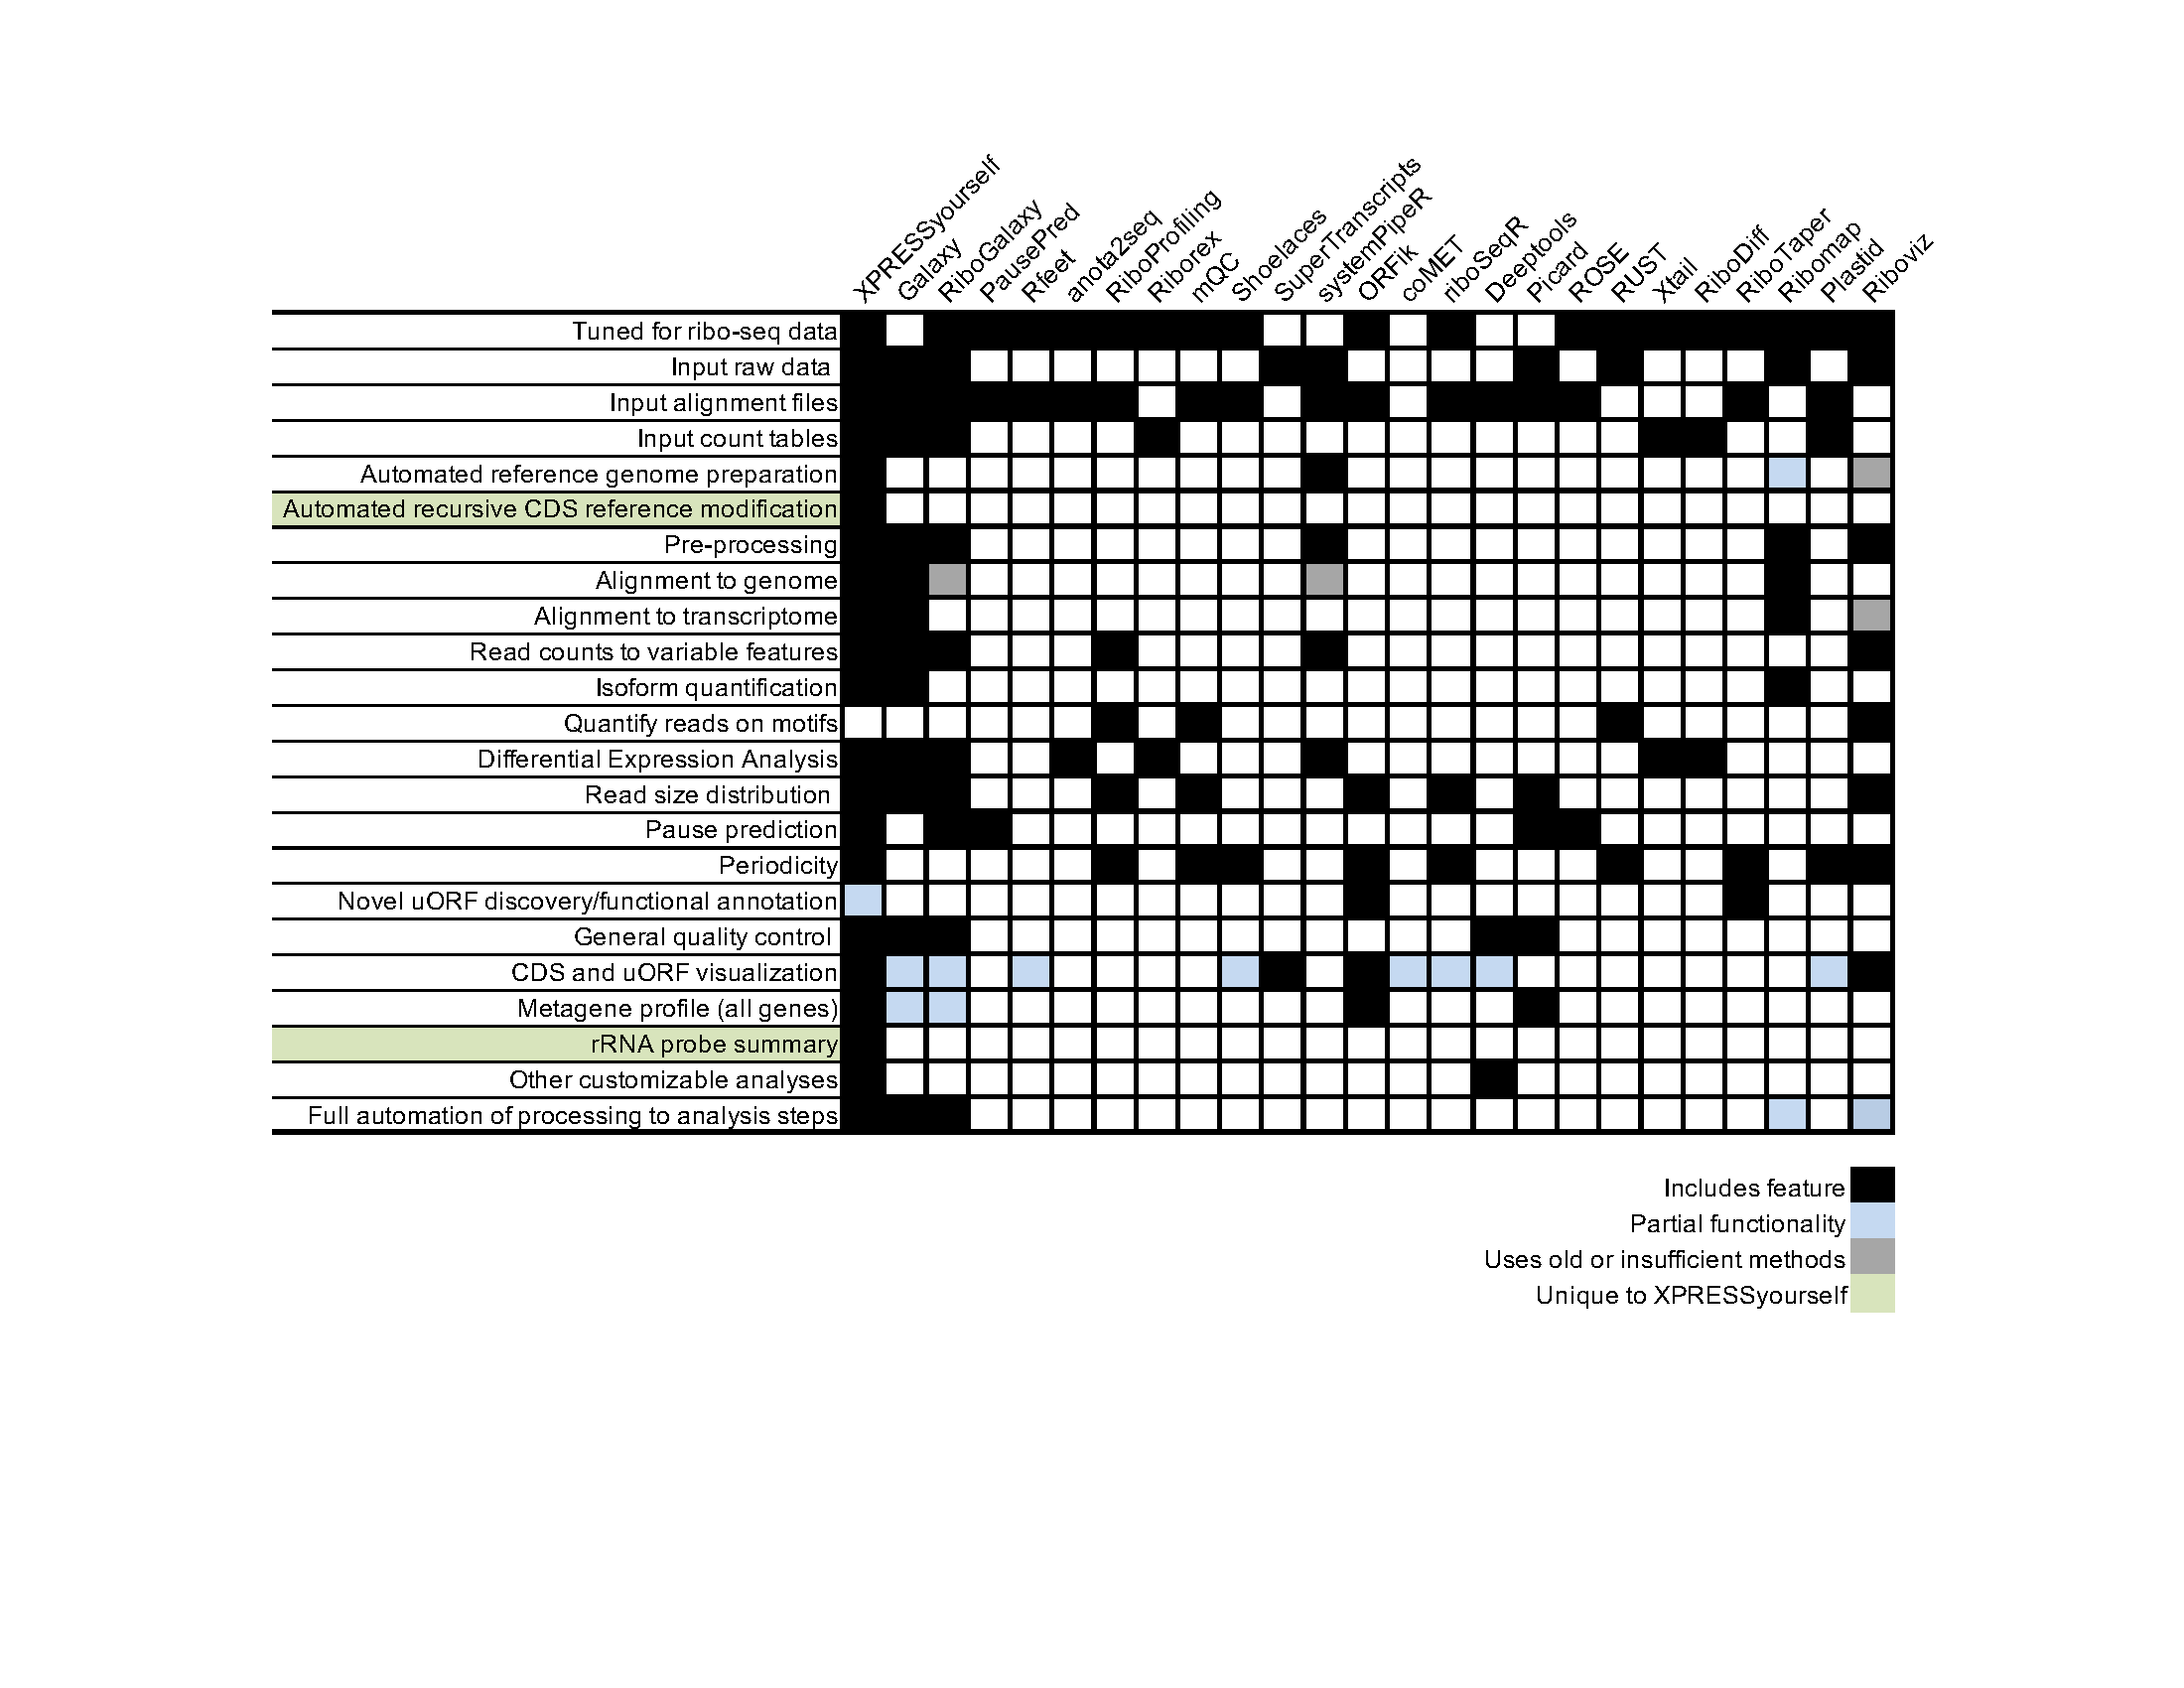
\includegraphics[width=160mm]{figures/xpresspipe_supplement1.png}
  \caption{\textbf{Comparison between IGV browser and geneCoverage output.} A) Gene coverage from IGV (above) and XPRESSpipe (below) for SLC1A1. B) Gene coverage from IGV (above) and XPRESSpipe (below) for TSPAN33. Introns collapsed by XPRESSpipe. Green box, region shown in corresponding IGV window comparing outputs between the two programs.}
  \label{fig:supplement1}
\end{figure}

\begin{figure}
\centering
  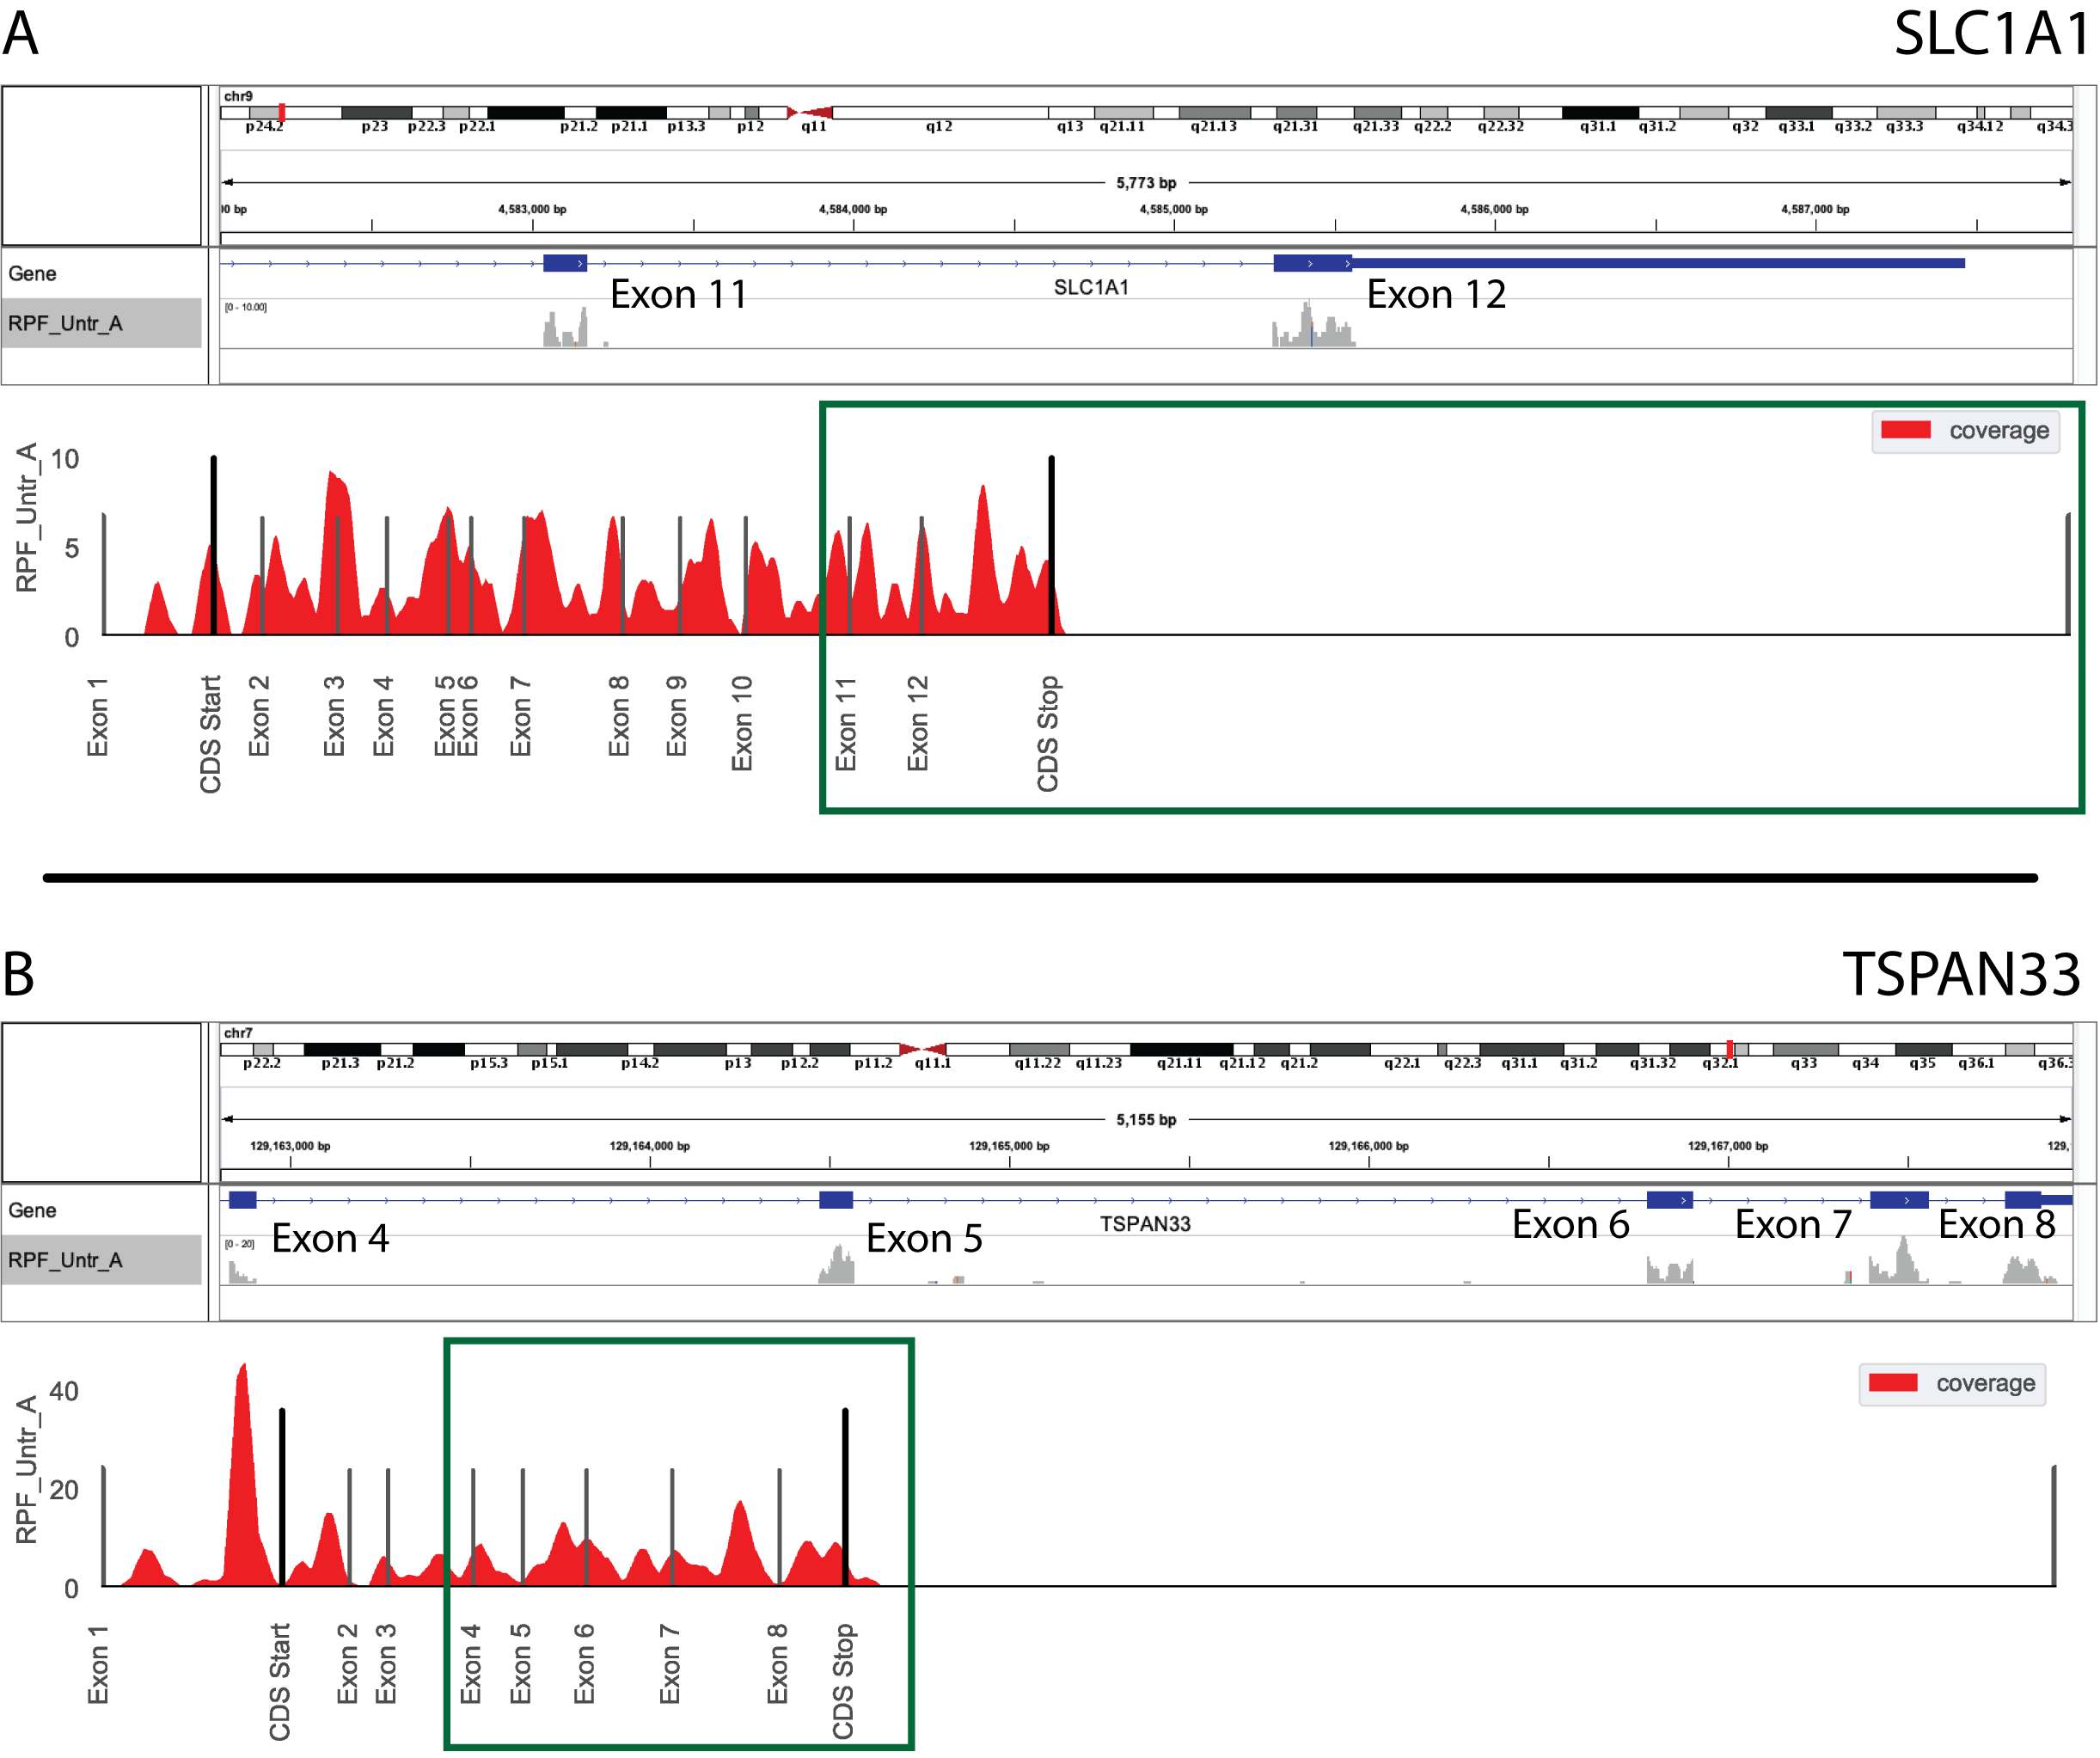
\includegraphics[width=160mm]{figures/xpresspipe_supplement2.png}
  \caption{\textbf{Original ISRIB count data plotted against XPRESSpipe-processed data reveals systematic differences between the analytical regimes.} A) Selected highlighted genes show consistent differences between processing methods. B) Spearman correlation plots using the data table provided as supplementary data with the original ISRIB manuscript comparing biological replicates. RPF, ribosome-protected footprint. Tm, tunicamycin. All $\rho$ values reported are Spearman correlation coefficients.}
  \label{fig:supplement2}
\end{figure}

\begin{figure}
\centering
  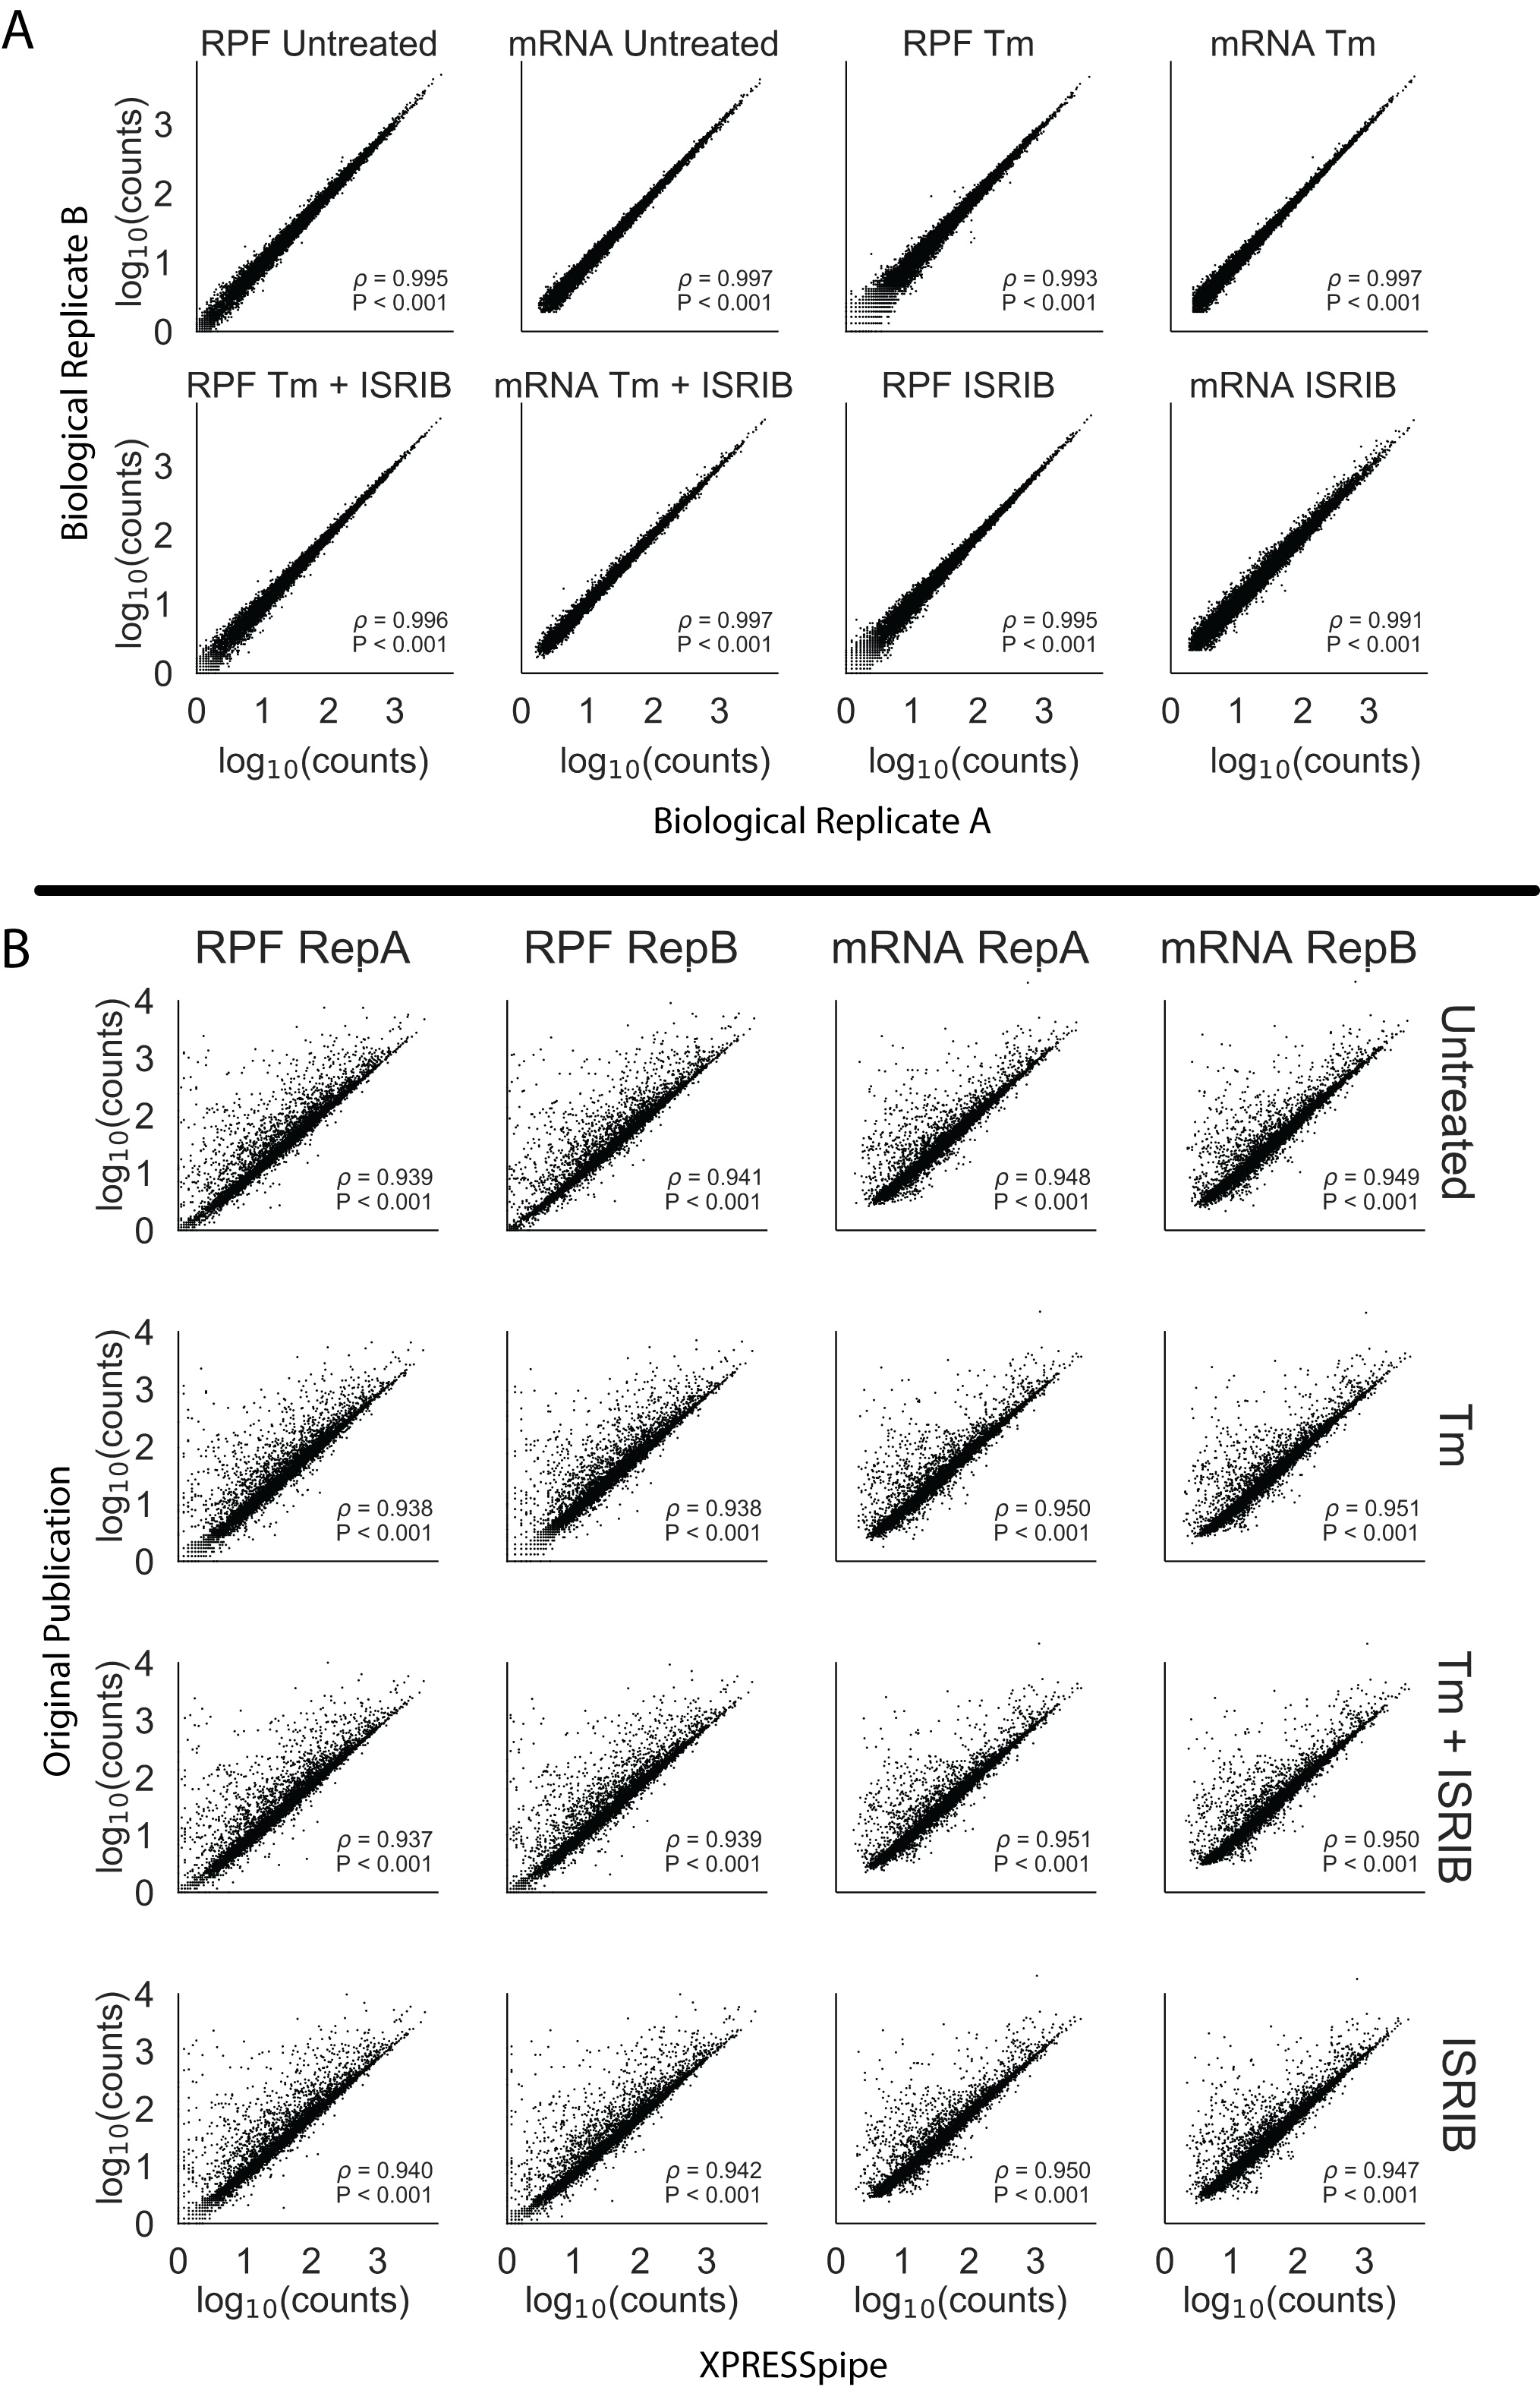
\includegraphics[width=180mm]{figures/xpresspipe_supplement3.png}
  \caption{\textbf{Original ISRIB count data plotted against XPRESSpipe-processed data quantifying with same reference version reveals negligible improvement in comparability between the analytical regimes.} Original samples were processed using Ensembl human build GRCh38 v72, as in the original manuscript, and compared with the original count data provided with the manuscript. XPRESSpipe-prepared counts were thresholded similarly as the original data (each gene needed to have at least 10 counts across all mRNA samples). RepA, biological replicate A. RepB, biological replicate B. RPF, ribosome-protected footprint. Tm, tunicamycin. All $\rho$ values reported are Spearman correlation coefficients.}
  \label{fig:supplement3}
\end{figure}

\begin{figure}
\centering
  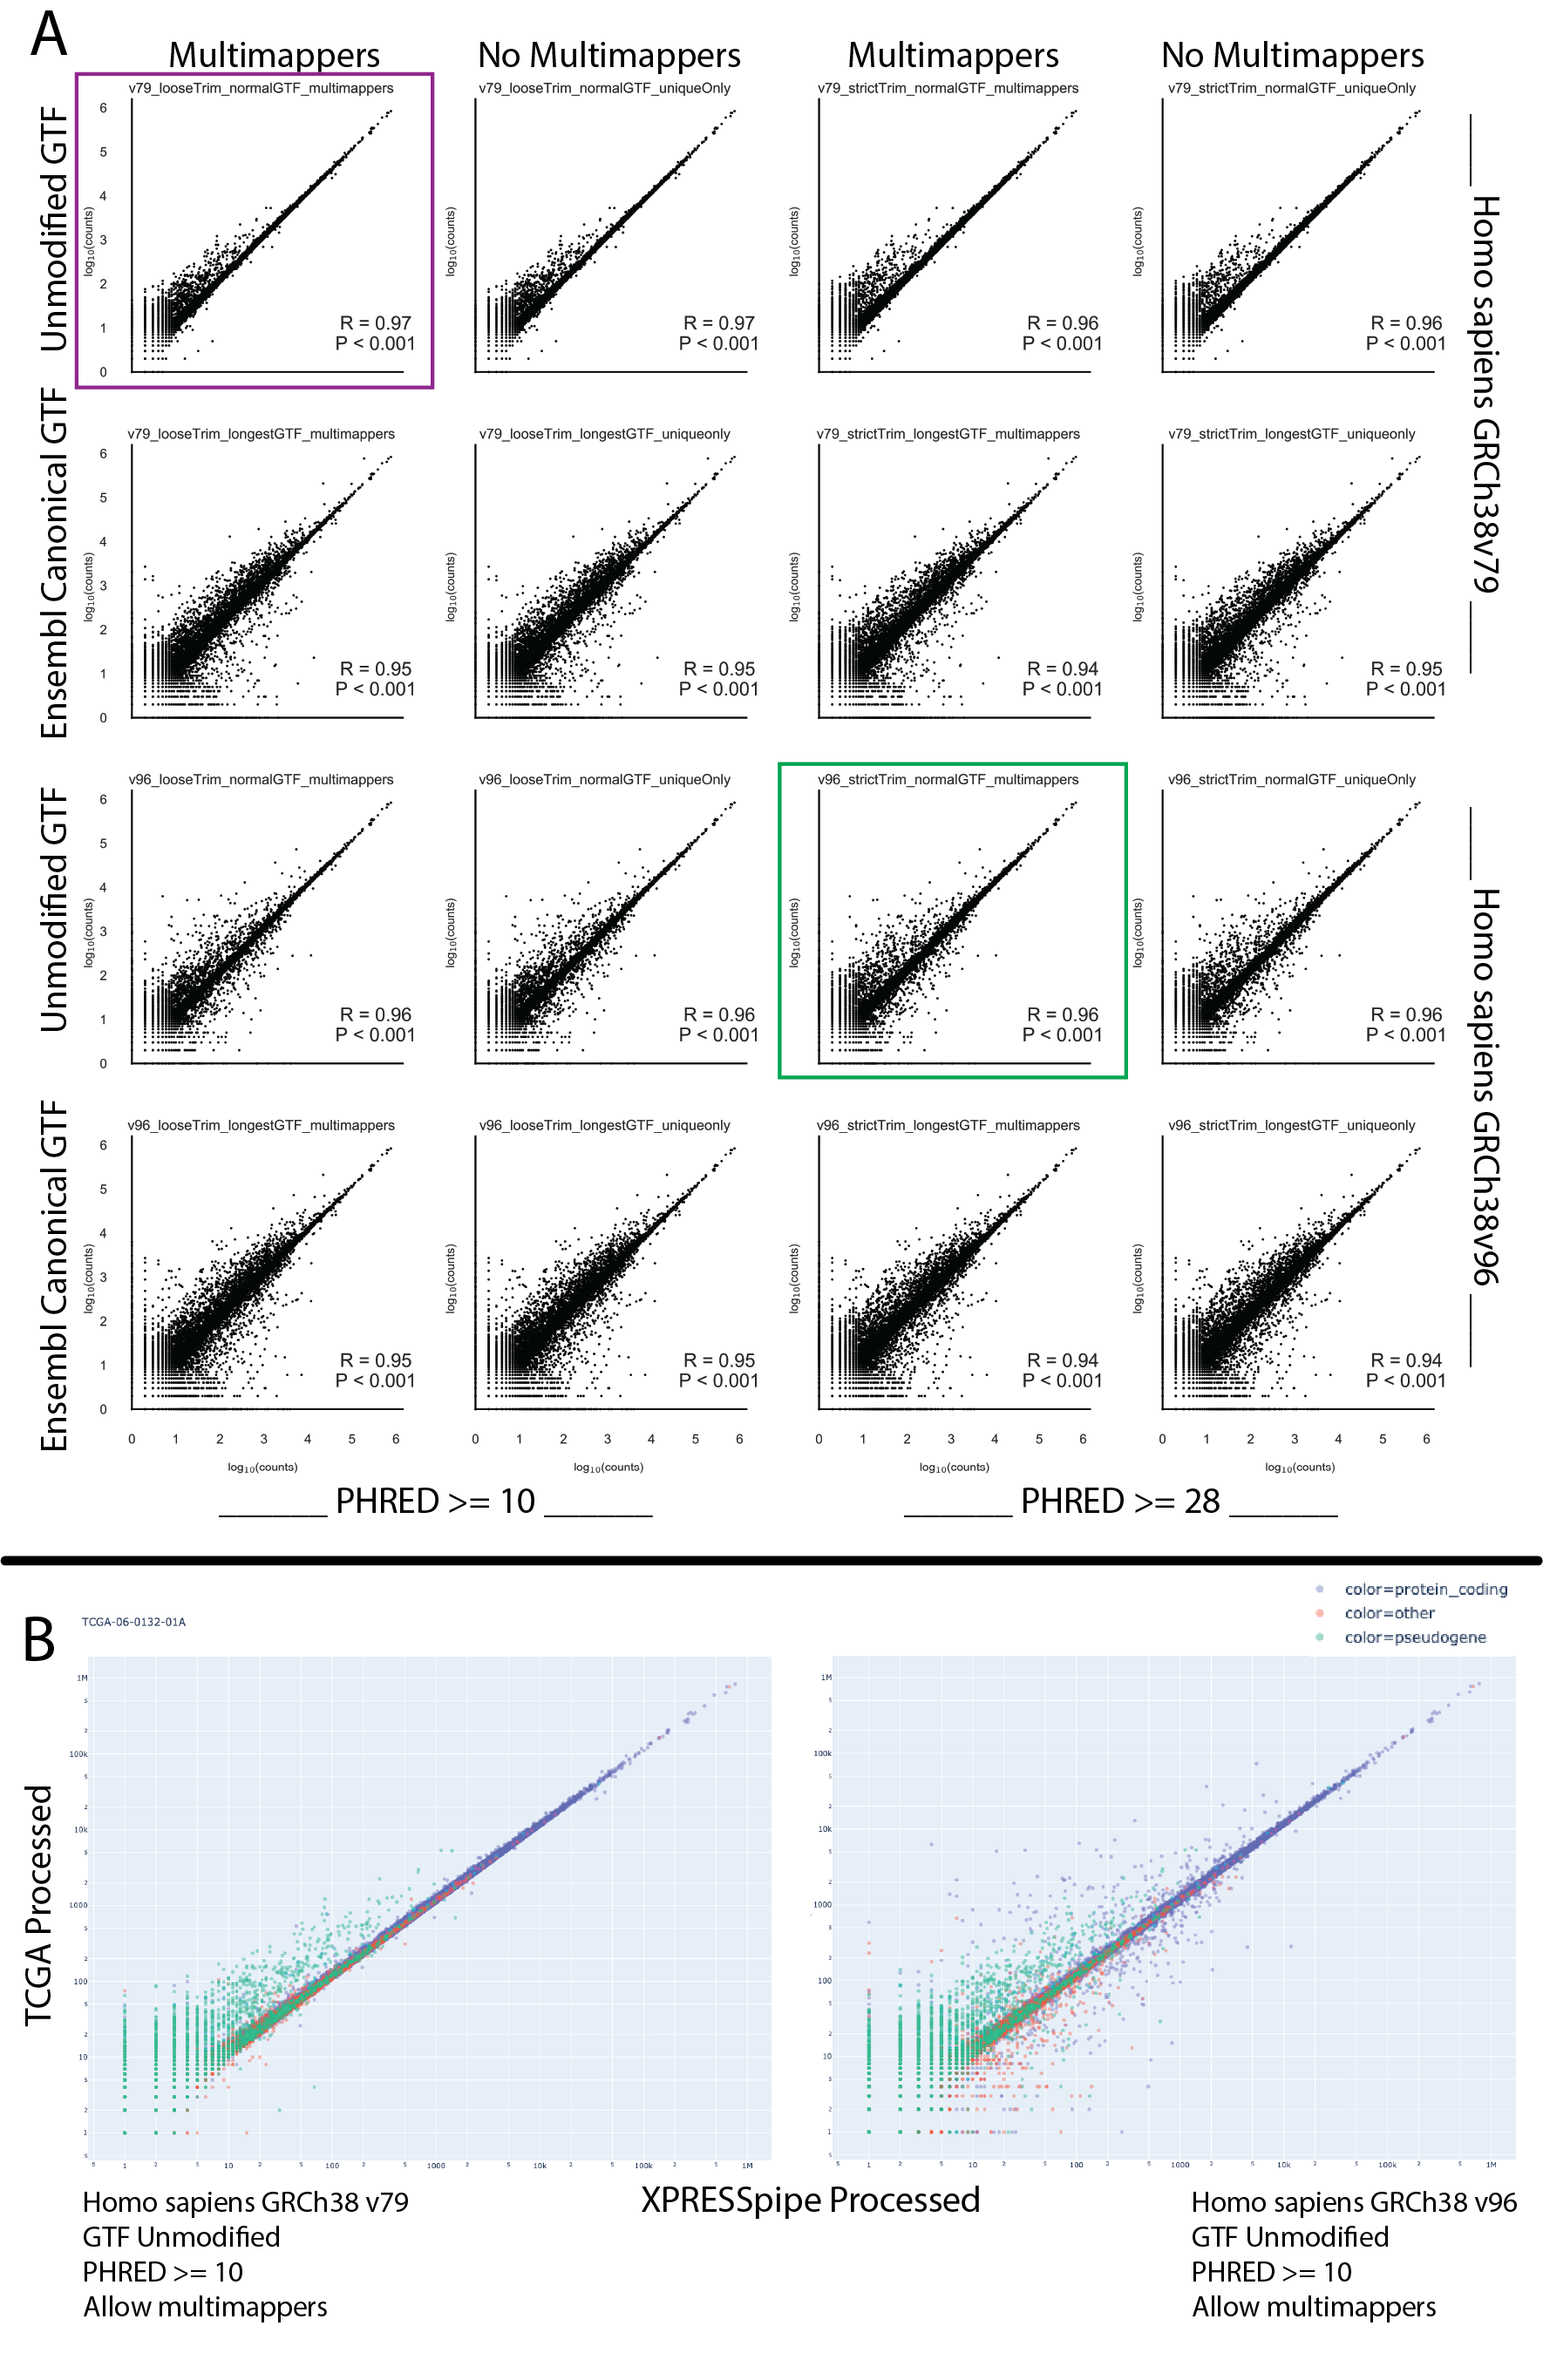
\includegraphics[width=180mm]{figures/xpresspipe_supplement4.png}
  \caption{\textbf{Gene coverage plots for neurologically annotated genes passing strict thresholding.} Coverage plots were generated using XPRESSpipe's geneCoverage module, which collapses introns within the representation.}
  \label{fig:supplement4}
\end{figure}

\begin{figure}
\centering
  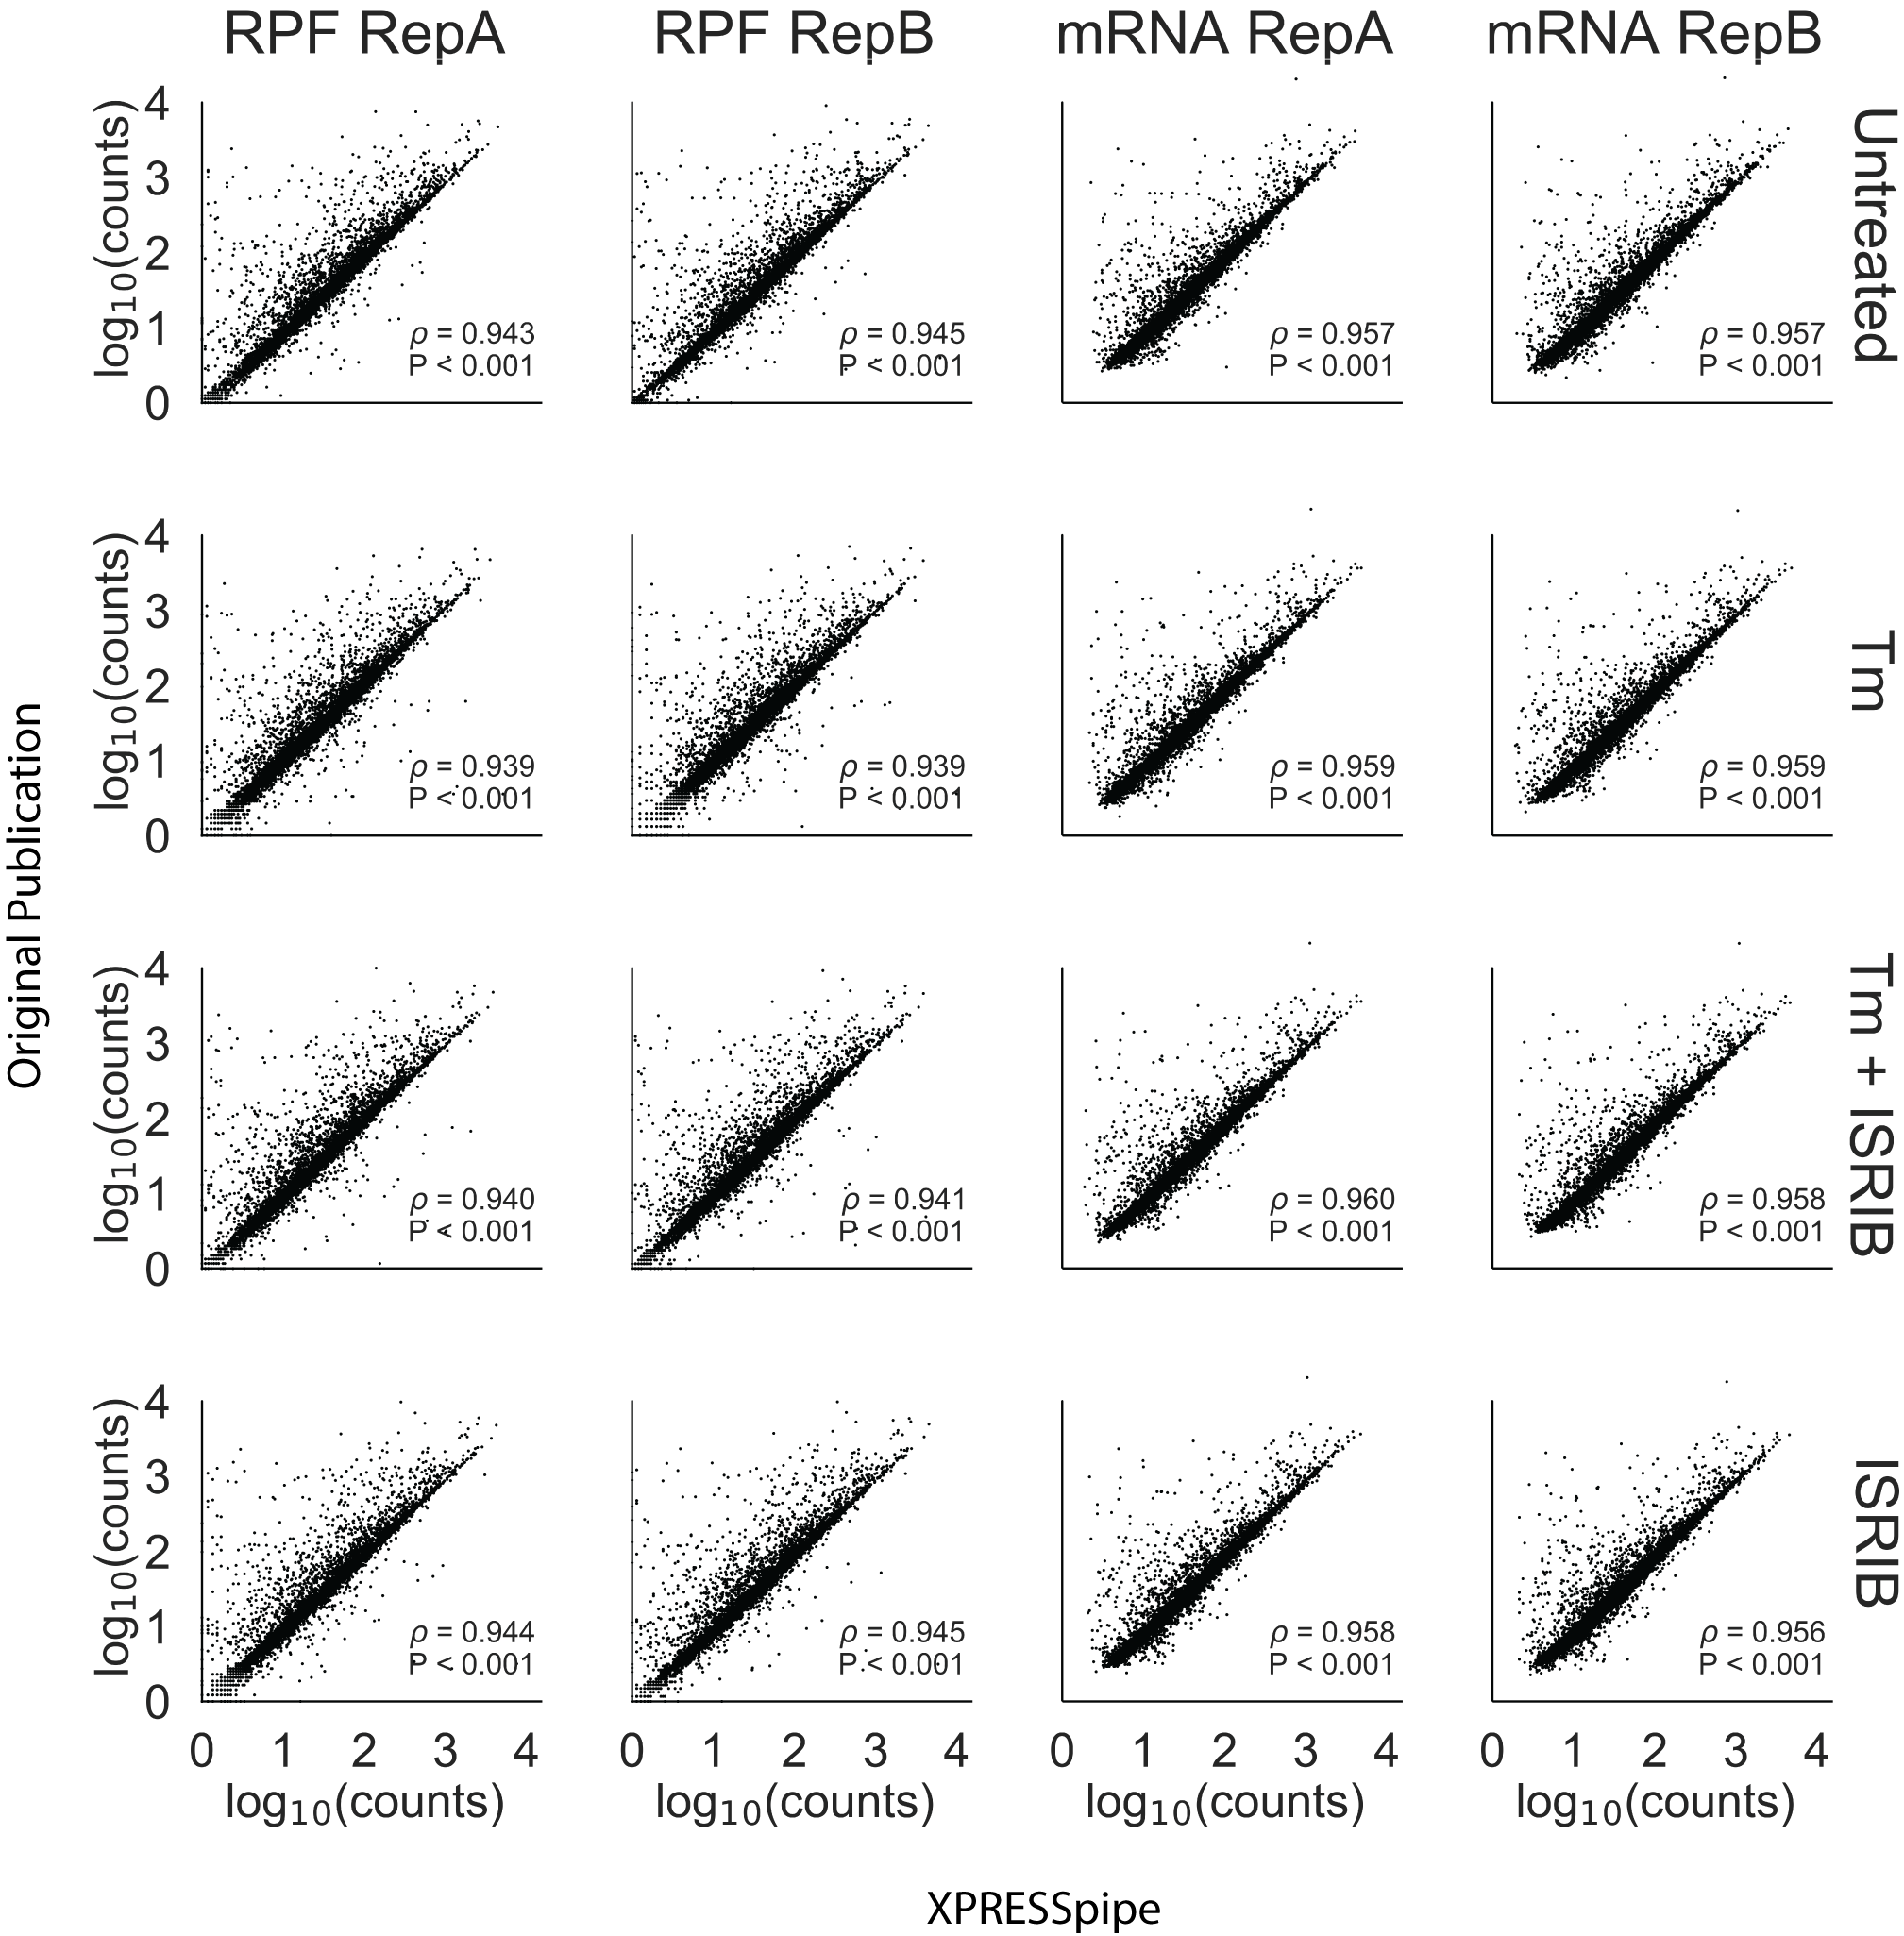
\includegraphics[width=180mm]{figures/xpresspipe_supplement5.png}
  \caption{\textbf{Sample RNA-Seq count data compared between TCGA count data and various conformations of the XPRESSpipe pipeline.} An overview of how different conformations of the XPRESSpipe peRNAseq pipeline compared to the published TCGA sample TCGA-06-0132-01A count data. The x-axis data in the plot enclosed in maroon most closely mirrors the settings used in the published TCGA RNA-Seq pipeline. The x-axis data in the plot enclosed in green used XPRESSpipe default settings and the most current reference transcriptome at the time of writing. All $\rho$ values reported are Spearman correlation coefficients.}
  \label{fig:supplement5}
\end{figure}

\begin{figure}
\centering
  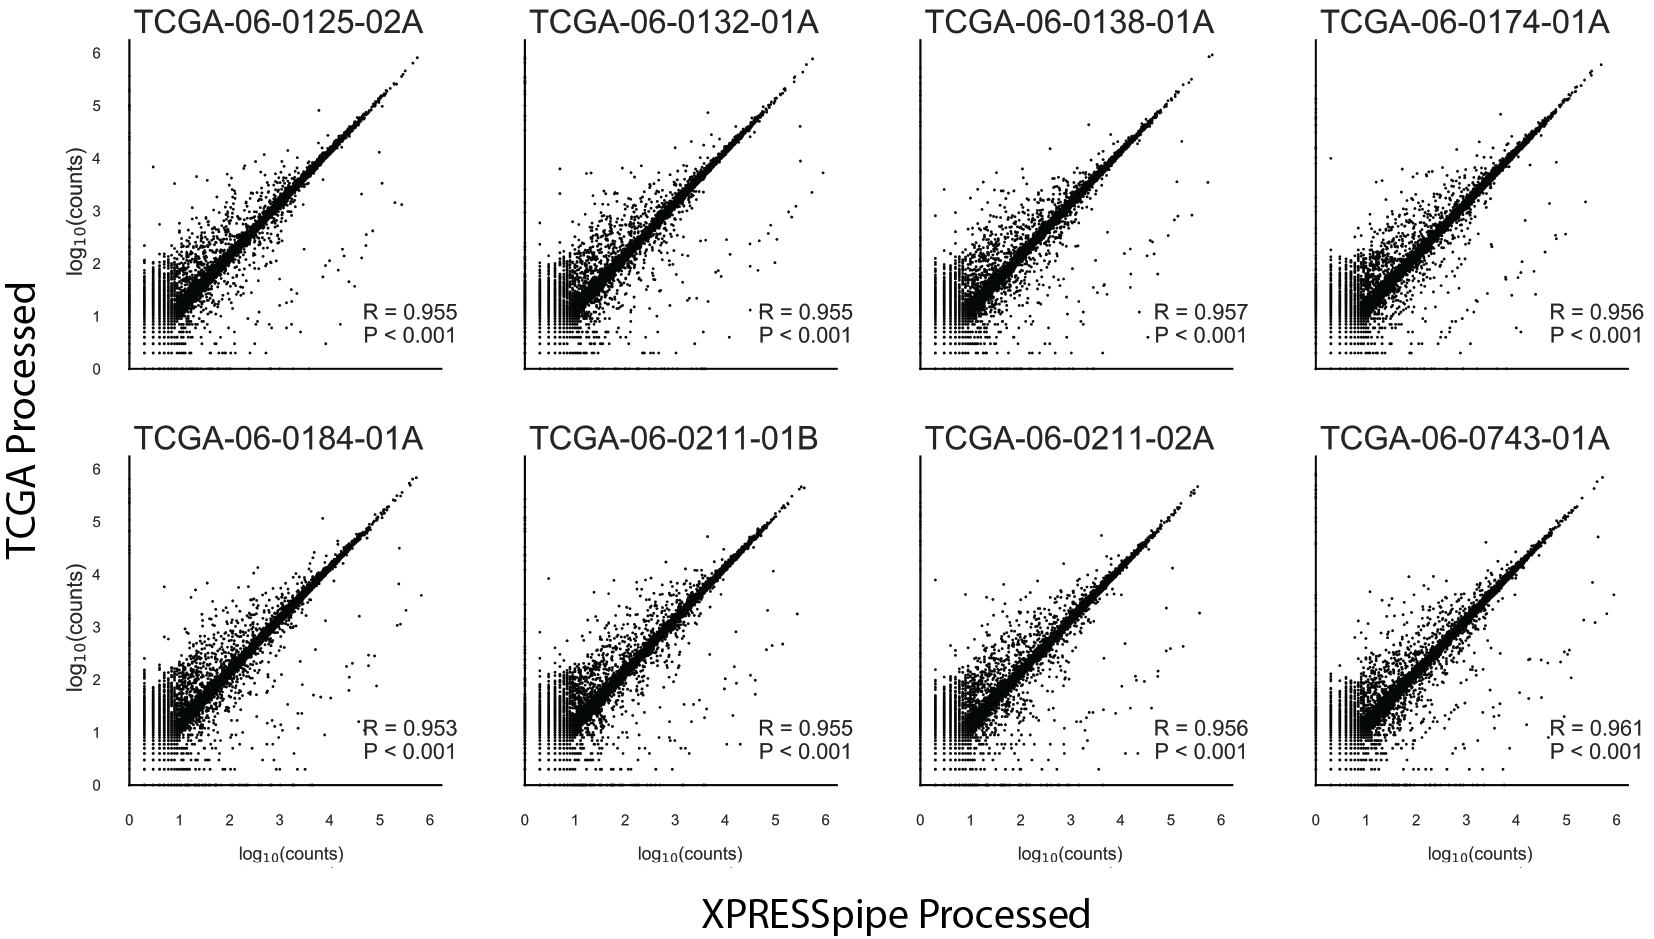
\includegraphics[width=180mm]{figures/xpresspipe_supplement6.png}
  \caption{\textbf{Effect of pseudogene inclusion on comparability between processing regimes.} Spearman correlations between XPRESSpipe and TCGA-processed count data with pseudogene counts included. All $\rho$ values reported are Spearman correlation coefficients.}
  \label{fig:supplement6}
\end{figure}

\begin{figure}
\centering
  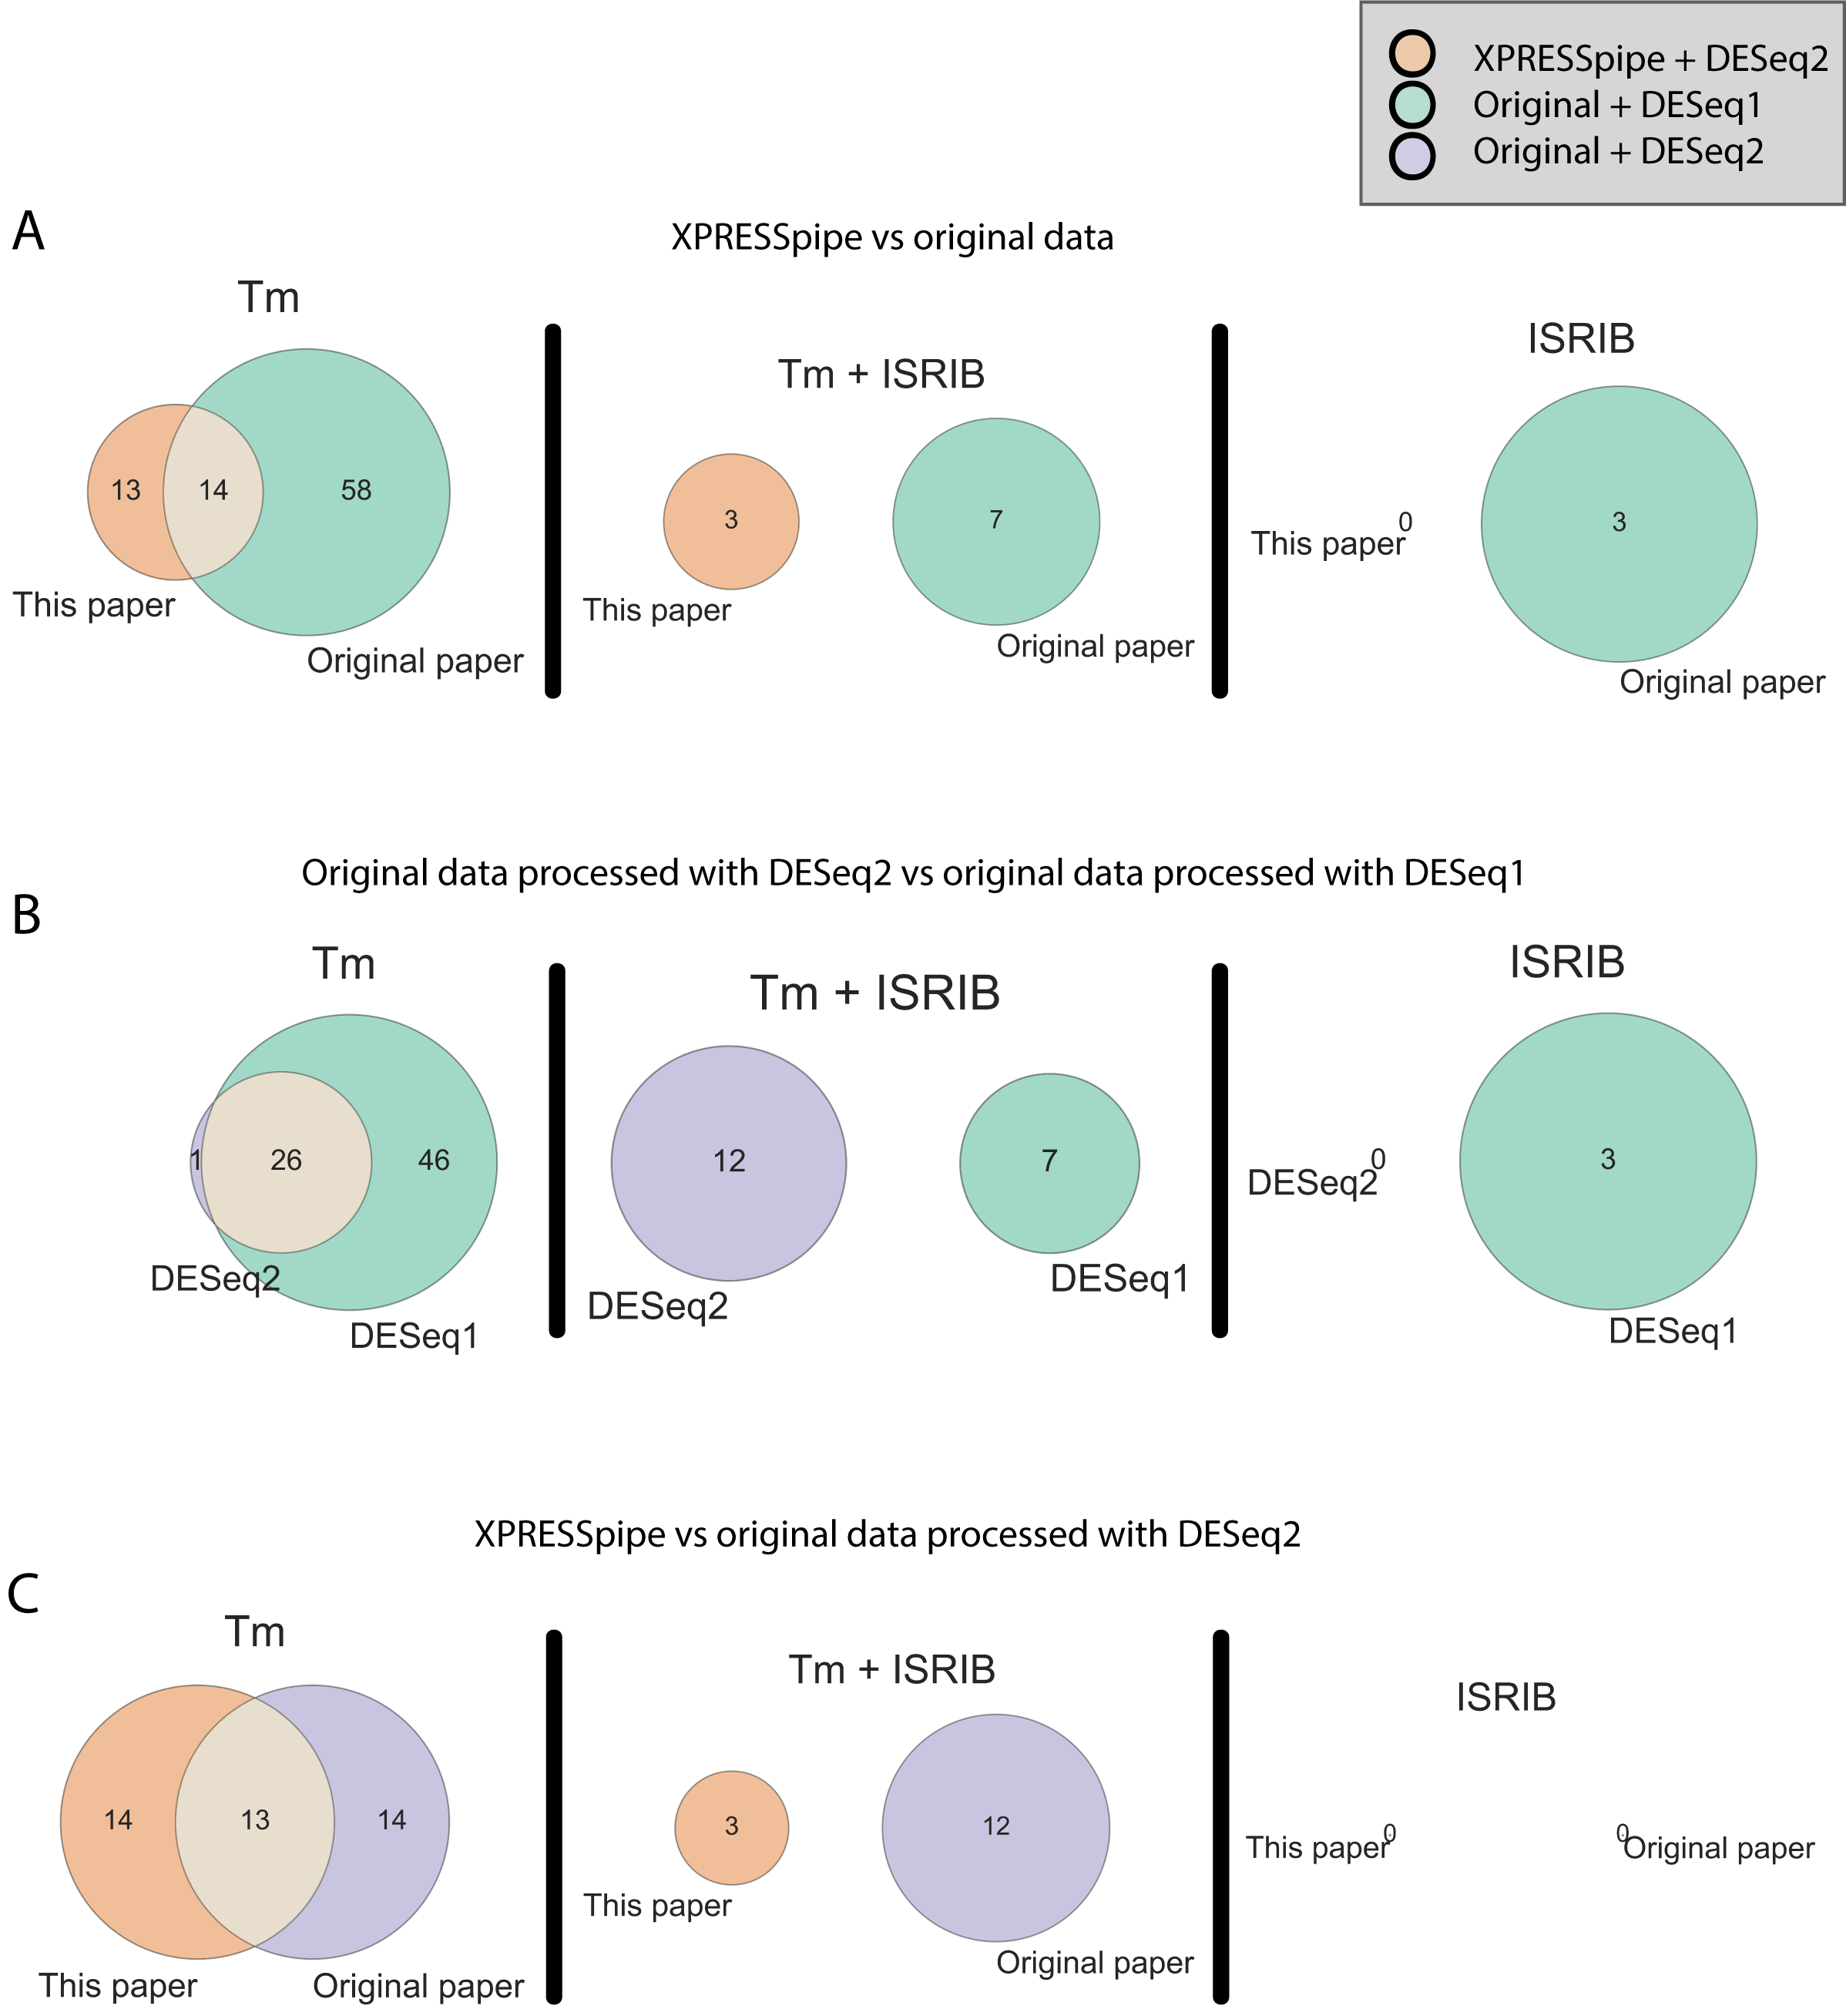
\includegraphics[width=180mm]{figures/xpresspipe_supplement7.png}
  \caption{\textbf{Removal of pseudogenes counts improve comparability between analytical regimes.} An overview of how different conformations of the XPRESSpipe peRNAseq pipeline compared to the published TCGA sample TCGA-06-0132-01A count data with pseudogenes collapsed. The x-axis data in the plot enclosed in maroon most closely mirrors the settings used in the published TCGA RNA-Seq pipeline. The x-axis data in the plot enclosed in green used XPRESSpipe default settings and a current reference transcriptome. All $\rho$ values reported are Spearman correlation coefficients.}
  \label{fig:supplement7}
\end{figure}

\begin{figure}
\centering
  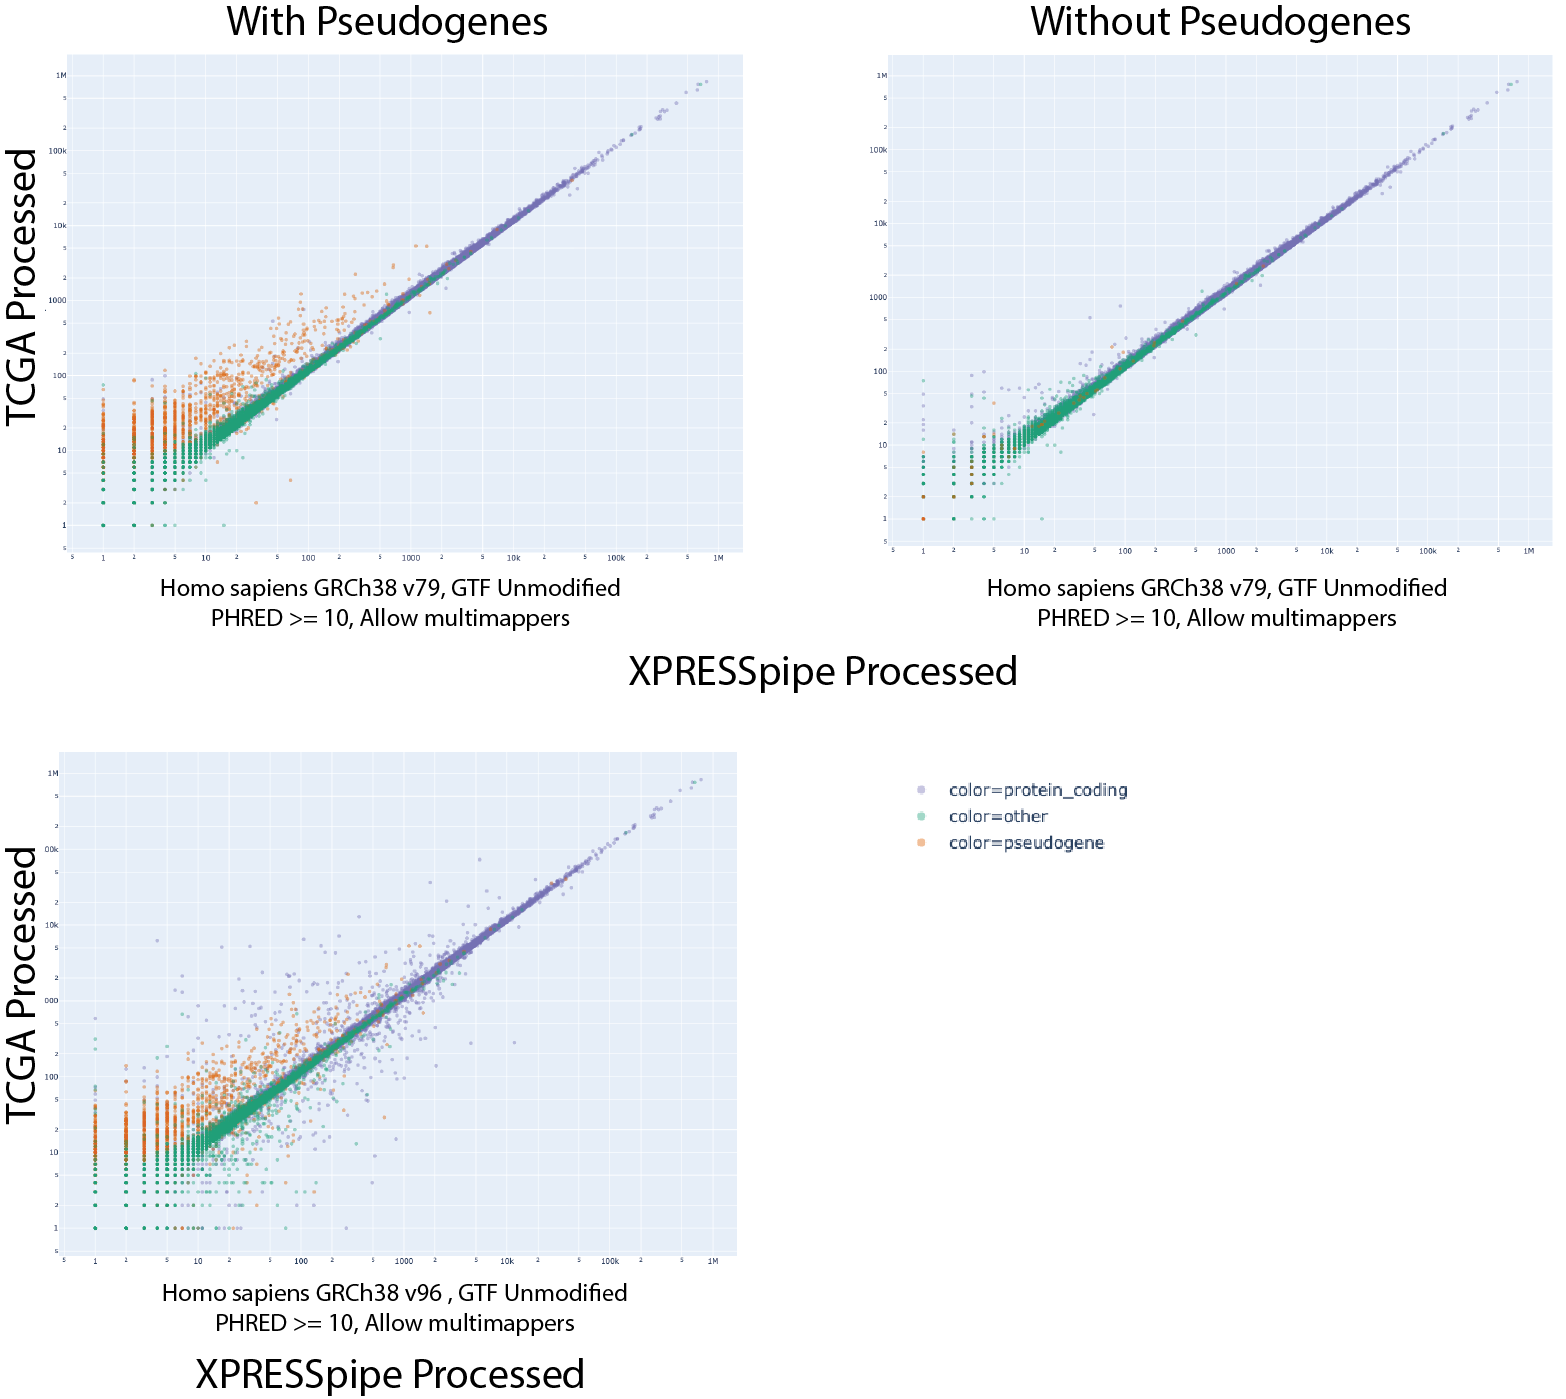
\includegraphics[width=180mm]{figures/xpresspipe_supplement8.png}
  \caption{\textbf{Pseudogenes counts are over-represented in TCGA-processed data.} An overview of gene-type distributions between transcriptome reference versions. The plots above used GRCh38v79 and the bottom plot used GRCh38v96. Purple points, protein-coding genes. Orange points, pseudogenes. Green points, other gene records. All plots represent sample TCGA-06-0132-01A and were processed the same way except for transcriptome reference used during read quantification.}
  \label{fig:supplement8}
\end{figure}

\end{document}
